% =====================================================================
% Rapport : Allocation dynamique de portefeuille par reinforcement learning
% Compilable avec pdfLaTeX (ex. Overleaf) ou XeLaTeX/Tectonic.
% Figures : générées par `python report/make_figures.py` (dossier figures/).
% =====================================================================
\documentclass[11pt,a4paper]{article}

\usepackage{iftex}
\ifPDFTeX
  \usepackage[utf8]{inputenc}
  \usepackage[T1]{fontenc}
  \usepackage{lmodern}
\else
  \usepackage{fontspec}
\fi
\usepackage[french]{babel}
\usepackage[margin=2.3cm]{geometry}
\usepackage{amsmath,amssymb}
\usepackage{graphicx}
\usepackage{booktabs}
\usepackage{tabularx}
\usepackage{array}
\usepackage{xcolor}
\usepackage{float}
\usepackage{caption}
\usepackage{enumitem}
\usepackage{listings}
\usepackage{algorithm}
\usepackage{algpseudocode}
\usepackage{tikz}
\usetikzlibrary{arrows.meta,positioning,shapes.geometric,fit,calc}
\usepackage[hidelinks]{hyperref}

\graphicspath{{figures/}}
\definecolor{bleu}{HTML}{2A78D6}
\definecolor{orange}{HTML}{EB6834}
\definecolor{vert}{HTML}{1BAF7A}
\definecolor{gris}{HTML}{52514E}
\definecolor{fond}{HTML}{F4F6FA}
\captionsetup{font=small,labelfont=bf}
\setlist{itemsep=2pt,topsep=4pt}
\newcolumntype{Y}{>{\raggedright\arraybackslash}X}
\lstset{basicstyle=\ttfamily\footnotesize, backgroundcolor=\color{fond}, frame=single, rulecolor=\color{gray!40},
        keywordstyle=\color{bleu}\bfseries, commentstyle=\color{gris}\itshape, columns=fullflexible,
        breaklines=true, language=Python, showstringspaces=false}
\floatname{algorithm}{Algorithme}
\renewcommand{\algorithmicrequire}{\textbf{Entrées :}}
\renewcommand{\algorithmicensure}{\textbf{Sortie :}}

\newcommand{\R}{\mathbb{R}}
\newcommand{\E}{\mathbb{E}}

\title{\textbf{Allocation dynamique de portefeuille\\par reinforcement learning}\\[4pt]
\large Application aux 50 actions de l'Euro Stoxx 50}
\author{Ayoub Hilal}
\date{Novembre 2026}

\begin{document}
\maketitle

\begin{abstract}
\noindent Ce projet construit un agent d'apprentissage par renforcement (\emph{Proximal Policy Optimization}, PPO)
qui décide chaque semaine de la répartition d'un portefeuille long-only entre les 50 actions de l'Euro Stoxx 50
et du cash. L'agent observe, pour chaque titre, des signaux documentés (momentum, retournement, volatilité,
drawdown) et le contexte de marché (tendance, volatilité, VIX) ; il ajuste un portefeuille de référence
(max-Sharpe) à l'aide d'un réseau de neurones partagé entre titres. Le protocole est strictement temporel :
les hyperparamètres sont choisis par validation glissante sur 2014--2021 (96 entraînements), puis le modèle
final est évalué une seule fois sur 2022--2026. Sur cette période, l'agent obtient un ratio de Sharpe de
\textbf{1,05} et un rendement de \textbf{16,5\,\%/an}, contre 0,65 et 10,0\,\%/an pour l'ETF Euro Stoxx 50
(dividendes inclus), avec une perte maximale plus faible (\(-18\,\%\) contre \(-21\,\%\)). L'analyse montre
toutefois que cette performance provient surtout de la conception (univers de 50 titres, portefeuille de
référence) et que l'apport propre de l'apprentissage reste faible : aucune différence avec les stratégies
diversifiées classiques n'est statistiquement significative.
\end{abstract}

\tableofcontents
\newpage

% =====================================================================
\section{Introduction}

\paragraph{Contexte.} L'allocation de portefeuille consiste à répartir un capital entre plusieurs actifs pour
obtenir le meilleur compromis rendement/risque. Les méthodes classiques (Markowitz, variance minimale, parité
de risque) estiment des moments statistiques puis résolvent un problème d'optimisation. L'apprentissage par
renforcement (RL) propose une approche différente : un \emph{agent} apprend directement, par interaction avec
un environnement simulé, une \emph{politique} qui associe à chaque état du marché une décision d'allocation,
en maximisant une récompense cumulée.

\paragraph{Objectif.} Construire de bout en bout un projet reproductible qui :
\begin{enumerate}
  \item récupère et nettoie les données des constituants de l'Euro Stoxx 50 (Yahoo Finance) ;
  \item formalise l'allocation hebdomadaire comme un processus de décision markovien ;
  \item entraîne un agent PPO et le compare honnêtement à des stratégies de référence, sous la même
        comptabilité (dates, frais, dérive des poids) ;
  \item respecte un protocole sans fuite d'information du futur, avec des tests statistiques.
\end{enumerate}

\paragraph{Contributions.} (i) Un environnement Gymnasium gérant un univers \emph{dynamique} (titres entrant
dans l'indice en cours de période) ; (ii) une politique PPO à \emph{réseau partagé entre titres},
équivariante par permutation ; (iii) un protocole de validation glissante avec réglage des hyperparamètres
et un test final verrouillé ; (iv) une évaluation statistique (intervalles de confiance du Sharpe par
bootstrap) et une analyse critique de l'apport de l'apprentissage.

% =====================================================================
\section{Le modèle en bref}

Avant d'entrer dans les détails, voici ce que fait le système, en termes simples.

\paragraph{Un gérant virtuel qui décide chaque vendredi.} Le modèle se comporte comme un gérant de portefeuille
qui, chaque vendredi soir, décide comment répartir l'argent entre les 50 actions de l'Euro Stoxx 50 et du cash
pour la semaine suivante. Il ne prédit pas les prix : il choisit une répartition et apprend, par expérience,
quelles répartitions donnent de bons résultats selon la situation.

\paragraph{Il part d'une recommandation éprouvée.} Plutôt que de partir de zéro, le gérant dispose chaque semaine
d'un portefeuille de référence calculé par une méthode classique de la finance, le \emph{max-Sharpe} : la
répartition qui, sur les trois dernières années, aurait offert le meilleur rendement pour le risque pris. Son rôle
est d'\textbf{ajuster} cette référence : renforcer certains titres, en alléger d'autres, et mettre une partie de
l'argent en cash (jusqu'à 50\,\%) s'il juge le marché dangereux.

\paragraph{Il regarde ce que regarde un analyste.} Pour chaque action, il observe des indicateurs simples :
a-t-elle plus monté que les autres sur un an, sur six mois ? A-t-elle chuté le mois dernier ? Est-elle plus agitée
que les autres ? Est-elle loin de son plus haut ? Il observe aussi l'humeur générale du marché : tendance de
l'indice, nervosité (volatilité, indice VIX).

\paragraph{Il apprend par essais et erreurs.} Pendant l'entraînement, le gérant « rejoue » des années passées
(2010--2021) des milliers de fois. Chaque semaine, il reçoit une note (la \emph{récompense}) : le gain de son
portefeuille, moins les frais de transaction, moins une pénalité si la semaine a été très agitée. Peu à peu, il
rend plus fréquentes les décisions qui ont obtenu de bonnes notes. C'est le principe de l'apprentissage par
renforcement ; l'algorithme utilisé s'appelle PPO.

\paragraph{Il est jugé sur des années qu'il n'a jamais vues.} Les réglages sont choisis sur 2014--2021, puis le
modèle final est évalué une seule fois sur 2022--2026, période qu'il n'a jamais vue pendant sa conception, et
comparé à l'ETF Euro Stoxx 50 et à sept stratégies classiques, dans exactement les mêmes conditions (mêmes dates,
mêmes frais).

\begin{figure}[H]
\centering
\begin{tikzpicture}[node distance=0.45cm, >=Stealth, every node/.style={font=\footnotesize},
  s/.style={draw=bleu, fill=fond, rounded corners, align=center, minimum width=2.45cm, minimum height=1.25cm, thick}]
  \node[s] (n1) {\textbf{1. Observer}\\ indicateurs des\\ 50 titres + marché};
  \node[s, right=of n1] (n2) {\textbf{2. Partir de}\\ \textbf{la référence}\\ max-Sharpe};
  \node[s, right=of n2] (n3) {\textbf{3. Ajuster}\\ renforcer, alléger,\\ mettre du cash};
  \node[s, right=of n3] (n4) {\textbf{4. Investir}\\ une semaine\\ (frais payés)};
  \node[s, right=of n4] (n5) {\textbf{5. Être noté}\\ gain $-$ frais\\ $-$ risque};
  \draw[->, thick] (n1) -- (n2); \draw[->, thick] (n2) -- (n3); \draw[->, thick] (n3) -- (n4); \draw[->, thick] (n4) -- (n5);
  \draw[->, thick, orange] (n5.south) -- ++(0,-0.55) -| node[pos=0.25, below]{à l'entraînement : la note sert à améliorer les décisions (apprentissage)} (n3.south);
\end{tikzpicture}
\caption{Une semaine du modèle.}
\label{fig:semaine}
\end{figure}

\paragraph{Le résultat en une phrase.} Sur 2022--2026, le modèle a rapporté \textbf{16,5\,\% par an} contre
\textbf{10,0\,\%} pour l'ETF Euro Stoxx 50, avec une perte maximale plus faible ; la section~\ref{sec:discussion}
explique honnêtement d'où vient cet écart et pourquoi ce modèle a été préféré aux stratégies classiques.

% =====================================================================
\section{Données}

\subsection{Sources et univers}
La composition actuelle de l'indice est extraite de la page Wikipédia \emph{EURO STOXX 50}
(\texttt{pandas.read\_html}). Chaque société est convertie en ticker Yahoo à partir de sa place de cotation
(Euronext Paris \(\to\) \texttt{.PA}, Xetra \(\to\) \texttt{.DE}, Euronext Amsterdam \(\to\) \texttt{.AS},
Borsa Italiana \(\to\) \texttt{.MI}, BME \(\to\) \texttt{.MC}, Nasdaq Helsinki \(\to\) \texttt{.HE},
Euronext Bruxelles \(\to\) \texttt{.BR}). Une liste de secours (\texttt{data/tickers\_fallback.csv}) est
utilisée si le scraping échoue ; chaque ticker est vérifié avec \texttt{yfinance}. Les 50 tickers ont été
résolus sans échec.

Sont téléchargés, du 2009-01-01 au 2026-11-20 (prix ajustés des dividendes et opérations sur titres,
\texttt{auto\_adjust=True}) :
\begin{itemize}
  \item les cours quotidiens et volumes des 50 actions ;
  \item deux benchmarks : l'indice \texttt{\^{}STOXX50E} (indice \emph{prix}, sans dividendes) et l'ETF
        \texttt{EXW1.DE} (iShares Core Euro Stoxx 50, dividendes réinvestis via les prix ajustés,
        environ +3\,\%/an par rapport à l'indice prix) ;
  \item le contexte de marché : l'indice et le VIX, depuis 2007.
\end{itemize}

\subsection{Nettoyage}
Les dates sont alignées sur un calendrier commun (union des jours de cotation), les valeurs manquantes
sont complétées par report de la dernière valeur sur au plus 3 jours, et les jours encore incomplets sont
supprimés. Le jeu final couvre \textbf{4\,583 jours} (2009-01-05 \(\to\) 2026-11-20), sans aucune valeur
manquante pour les titres cotés. Un rapport (\texttt{data/processed/report.md}) liste les tickers, les
retraits et leurs raisons.

\subsection{Univers dynamique}
Cinq sociétés sont entrées en bourse après 2009 : Argenx (2014), Ferrari (2016), Adyen (2018), Prosus (2019)
et Siemens Energy (2020). Plutôt que de les exclure, le modèle les rend \textbf{investissables un an après
leur première cotation}, dès que tous leurs signaux sont calculables avec leurs seuls prix passés. Un
\emph{masque de disponibilité} \(m_{t,i}\in\{0,1\}\) est propagé dans l'environnement, les stratégies de
référence et le réseau de neurones : un titre indisponible a toujours un poids nul et n'influence pas les
décisions. La figure~\ref{fig:univers} montre l'évolution de l'univers investissable (45 titres en 2010,
50 à partir de fin 2021).

\begin{figure}[H]
  \centering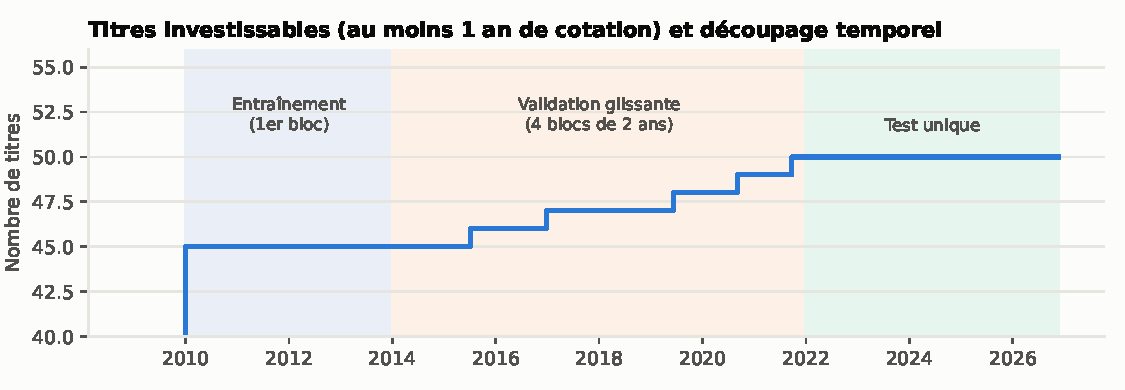
\includegraphics[width=\linewidth]{fig_univers}
  \caption{Nombre de titres investissables et découpage temporel du protocole.}
  \label{fig:univers}
\end{figure}

\subsection{Calendrier de décision et découpage temporel}
Les décisions sont \textbf{hebdomadaires}, prises au dernier jour de bourse de chaque semaine ; les poids
choisis à la date \(t_k\) s'appliquent aux rendements de la période \((t_k,t_{k+1}]\). Une période n'appartient
à un ensemble (entraînement, validation, test) que si la décision \emph{et} la fin de la période de détention y
sont incluses : aucune semaine n'est à cheval sur deux ensembles. Le test couvre \textbf{254 semaines}
(2022-01-07 \(\to\) 2026-11-13).

% =====================================================================
\section{Formulation du problème d'apprentissage par renforcement}\label{sec:formulation}

\subsection{Vocabulaire du reinforcement learning}
Un problème d'apprentissage par renforcement met en jeu un \textbf{agent} qui interagit avec un
\textbf{environnement} à intervalles réguliers. À chaque instant \(t\) :
\begin{enumerate}
  \item l'environnement est dans un \textbf{état} \(s_t\) (tout ce que l'agent sait au moment de décider) ;
  \item l'agent choisit une \textbf{action} \(a_t\) selon sa \textbf{politique} \(\pi\), c'est-à-dire sa règle
        de décision ;
  \item l'environnement évolue vers un nouvel état \(s_{t+1}\) et renvoie une \textbf{récompense} \(r_t\),
        un nombre qui mesure la qualité de la décision.
\end{enumerate}
L'objectif de l'agent est de trouver la politique qui rend les récompenses les plus grandes possible en
moyenne. Ce cadre est formalisé par un \emph{processus de décision markovien}
\((\mathcal S,\mathcal A,P,r,\gamma)\) : un ensemble d'états \(\mathcal S\), un ensemble d'actions
\(\mathcal A\), une dynamique \(P(s_{t+1}\mid s_t,a_t)\) (comment l'état évolue), une fonction de récompense
\(r\) et un facteur d'actualisation \(\gamma\in[0,1]\) (le poids donné aux récompenses futures).

Dans ce projet, une \textbf{étape \(t\) correspond à une semaine} : l'agent décide de la composition du
portefeuille le dernier jour de bourse de la semaine \(t\), et cette composition s'applique aux rendements de la
semaine suivante. La figure~\ref{fig:boucle} résume la boucle, implémentée dans \texttt{src/env.py}
(classe \texttt{PortfolioEnv}, interface Gymnasium).

\begin{figure}[H]
\centering
\begin{tikzpicture}[node distance=1.2cm and 2.4cm, >=Stealth, every node/.style={font=\small},
  box/.style={draw=bleu, fill=fond, rounded corners, minimum width=3.6cm, minimum height=1.1cm, align=center, thick}]
  \node[box] (agent) {\textbf{Agent PPO}\\ politique \(\pi_\theta(a\mid s)\)};
  \node[box, right=4.2cm of agent] (env) {\textbf{Environnement}\\ marché + comptabilité};
  \draw[->, thick, bleu] (agent.north) to[bend left=25] node[above]{action \(a_t\) : une note par titre + une pour le cash} (env.north);
  \draw[->, thick, orange] (env.south) to[bend left=25] node[below]{nouvel état \(s_{t+1}\), récompense \(r_t\)} (agent.south);
\end{tikzpicture}
\caption{Boucle hebdomadaire entre l'agent et l'environnement de marché.}
\label{fig:boucle}
\end{figure}

\subsection{Notations}
Le tableau~\ref{tab:notations} rassemble tous les symboles utilisés dans les sections~\ref{sec:formulation} et~\ref{sec:ppo}.

\begin{table}[H]
\centering\small
\caption{Notations (les valeurs sont celles du modèle retenu, fichier \texttt{config.yaml}).}
\label{tab:notations}
\begin{tabularx}{\linewidth}{@{}lYl@{}}
\toprule
Symbole & Signification & Valeur\\
\midrule
\multicolumn{3}{@{}l}{\emph{Marché et portefeuille}}\\
\(t\) & indice de la semaine (étape de décision) & --\\
\(N\) & nombre de titres de l'univers & 50\\
\(i\) & indice d'un titre, \(i=1,\dots,N\) ; l'indice « cash » désigne la liquidité & --\\
\(m_{t,i}\) & disponibilité du titre \(i\) en \(t\) (1 s'il a au moins un an de cotation, 0 sinon) & 0 ou 1\\
\(R_{t,i}\) & rendement du titre \(i\) pendant la semaine qui suit la décision \(t\) & --\\
\(w_{t,i}\) & poids du titre \(i\) \emph{après} la décision \(t\) (part du capital) ; \(\sum_i w_{t,i}+w_{t,\text{cash}}=1\) & --\\
\(w^{-}_{t,i}\) & poids \emph{avant} la décision \(t\), après la dérive des prix de la semaine précédente & --\\
\(b_{t,i}\) & poids du portefeuille de référence (max-Sharpe) en \(t\) & --\\
\(V_t\) & valeur du portefeuille en \(t\) (base 1 au départ) & --\\
\midrule
\multicolumn{3}{@{}l}{\emph{Environnement}}\\
\(s_t\) & état observé par l'agent en \(t\) & \(\in\R^{751}\)\\
\(x_{t,i}\) & vecteur des 14 informations du titre \(i\) (signaux, contexte, disponibilité) & \(\in\R^{14}\)\\
\(a_t\) & action : une note \(a_{t,i}\in[-1,1]\) par titre, plus une note \(a_{t,\text{cash}}\) & \(\in[-1,1]^{51}\)\\
\(\tilde w_t\) & poids cibles déduits de l'action & --\\
\(\kappa\) & intensité des inclinaisons autour de la référence & 1\\
\(\varepsilon\) & plancher ajouté aux poids de référence & 0,002\\
\(c_{\max}\) & part maximale de cash & 50\,\%\\
\(\alpha\) & vitesse de lissage (part du chemin parcourue vers la cible chaque semaine) & 0,5\\
\(c\) & coût de transaction par unité échangée (performance mesurée) & 0,1\,\%\\
\(c_{\text{train}}\) & coût utilisé dans la récompense d'entraînement & 0,3\,\%\\
\(\gamma_{\text{r}}\) & aversion au risque de la récompense & 2\\
\(r_t\) & récompense de l'étape \(t\) & --\\
\midrule
\multicolumn{3}{@{}l}{\emph{Agent et apprentissage}}\\
\(\pi_\theta(a\mid s)\) & politique : loi de probabilité de l'action \(a\) dans l'état \(s\) & --\\
\(\theta\) & paramètres de la politique (poids du réseau, écarts-types d'exploration) & --\\
\(\mu_\theta(s)\), \(\sigma\) & moyenne et écarts-types de la loi normale des actions & \(\log\sigma_0=-0{,}5\)\\
\(V_\phi(s)\) & fonction de valeur estimée (critique), de paramètres \(\phi\) & --\\
\(\gamma\) & facteur d'actualisation des récompenses futures & 0\\
\(\hat A_t\) & avantage estimé de l'action \(a_t\) & --\\
\(\rho_t(\theta)\) & ratio de probabilité entre la nouvelle et l'ancienne politique & --\\
\(\epsilon\) & seuil de découpage (« clipping ») de PPO & 0,2\\
\(\lambda\) & paramètre de l'estimateur d'avantage GAE & 0,95\\
\(c_v\), \(c_e\) & poids de l'erreur de valeur et du bonus d'entropie dans la perte & 0,5 ; 0,005\\
\(\eta\) & taux d'apprentissage de l'optimiseur Adam & \(3\cdot10^{-4}\to0\)\\
\bottomrule
\end{tabularx}
\end{table}

\subsection{État \(s_t\) : ce que voit l'agent}\label{sec:etat}
Pour chaque titre \(i\), le vecteur \(x_{t,i}\in\R^{14}\) contient uniquement des informations connues à la date
\(t\) :
\begin{itemize}
  \item \textbf{6 rangs} dans \([-1,1]\) parmi les titres disponibles (\(-1\) : le plus faible, \(+1\) : le plus
        fort) : momentum 12-1 (rendement entre \(t-12\) mois et \(t-1\) mois), momentum 6-1, retournement à 1 mois
        (rendement du dernier mois), rendement de la dernière semaine, volatilité sur 60 jours, drawdown sur
        252 jours (distance au plus haut de l'année) ;
  \item \textbf{2 signaux en niveau} : momentum 12-1 et volatilité du titre ;
  \item \textbf{5 variables de contexte de marché}, identiques pour tous les titres : écart de l'indice à sa
        moyenne mobile 200 jours (tendance), volatilité de l'indice sur 20 jours, rendement de l'indice sur
        13 semaines, niveau du VIX et sa variation sur 20 jours ;
  \item \textbf{le drapeau de disponibilité} \(m_{t,i}\).
\end{itemize}
Chaque variable (sauf le drapeau) est centrée-réduite avec la moyenne et l'écart-type calculés
\emph{uniquement sur la période d'entraînement}, puis écrêtée à \(\pm5\). L'état complet juxtapose les 50 vecteurs
\(x_{t,i}\) et les 51 poids courants \(w^{-}_{t}\) : \(s_t\in\R^{50\times14+51}=\R^{751}\).

\subsection{Action \(a_t\) et poids du portefeuille}\label{sec:action}
L'action contient 51 notes dans \([-1,1]\). Elles sont transformées en poids en trois étapes.

\paragraph{1. Part de cash.} \(c_t=c_{\max}\cdot\max(a_{t,\text{cash}},0)\) : une note de cash négative ou nulle
signifie 0\,\% de cash, une note de \(+1\) signifie 50\,\%.

\paragraph{2. Répartition entre titres.} Le reste, \(1-c_t\), est réparti par une fonction \emph{softmax}
(qui transforme des scores en proportions positives de somme 1) appliquée aux notes, décalées par le portefeuille
de référence :
\begin{equation}
  \tilde w_{t,i}=(1-c_t)\,\frac{m_{t,i}\,\exp\!\big(\kappa\,a_{t,i}+\log(b_{t,i}+\varepsilon)\big)}
  {\sum_{j=1}^{N} m_{t,j}\,\exp\!\big(\kappa\,a_{t,j}+\log(b_{t,j}+\varepsilon)\big)}
  =(1-c_t)\,\frac{m_{t,i}\,(b_{t,i}+\varepsilon)\,e^{\kappa a_{t,i}}}{\sum_{j} m_{t,j}\,(b_{t,j}+\varepsilon)\,e^{\kappa a_{t,j}}}.
\end{equation}
\emph{Lecture} : si toutes les notes valent 0, on retrouve le portefeuille de référence (à \(\varepsilon\) près).
Une note \(a_{t,i}=+1\) multiplie le poids relatif du titre \(i\) par \(e\approx2{,}7\) ; une note de \(-1\) le divise
par \(2{,}7\). Le facteur \(m_{t,i}\) annule le poids des titres indisponibles, et \(\varepsilon\) permet d'investir
dans un titre auquel la référence n'attribue rien.

\paragraph{3. Lissage.} Le portefeuille ne fait que la moitié du chemin vers la cible :
\(w_t=(1-\alpha)\,w^{-}_t+\alpha\,\tilde w_t\), avec \(\alpha=0{,}5\). Cela limite les échanges, donc les frais.

\paragraph{Exemple chiffré.} Avec trois titres de poids de référence \((0{,}5;\ 0{,}3;\ 0{,}2)\), sans cash et des
notes \((+1;\ 0;\ -1)\), les poids relatifs deviennent \(0{,}5e\), \(0{,}3\) et \(0{,}2/e\), soit après normalisation
\((0{,}78;\ 0{,}17;\ 0{,}04)\) : l'agent a renforcé le premier titre et allégé le troisième.

\subsection{Dynamique : comptabilité d'une semaine}
Une fois les poids \(w_t\) fixés, la semaine se déroule ainsi :
\begin{align}
  \text{turnover}_t &= \sum_{i=1}^{N}\big|w_{t,i}-w^{-}_{t,i}\big|
  &&\text{(part du portefeuille échangée ; la jambe cash est gratuite)}\\
  R^{\text{brut}}_t &= \sum_{i} w_{t,i}\,R_{t,i} + w_{t,\text{cash}}\,R_{t,\text{cash}}
  &&\text{(rendement du portefeuille avant frais)}\\
  r^{\text{net}}_t &= R^{\text{brut}}_t - c\cdot\text{turnover}_t
  &&\text{(rendement net de frais)}\\
  V_{t+1} &= V_t\,(1+r^{\text{net}}_t)
  &&\text{(valeur du portefeuille)}\\
  w^{-}_{t+1,i} &= \frac{w_{t,i}\,(1+R_{t,i})}{1+R^{\text{brut}}_t}
  &&\text{(dérive : un titre qui monte pèse plus lourd)}
\end{align}
Le cash rapporte \(R_{t,\text{cash}}=0\). Cette comptabilité est écrite une seule fois (fonction
\texttt{rebalance\_step}) et utilisée à l'identique par l'agent et par toutes les stratégies de référence :

\begin{lstlisting}
def rebalance_step(w_prev, w_new, asset_returns, cost_rate, include_cash=True):
    delta = np.abs(w_new - w_prev)
    turnover = delta.sum() if include_cash else delta[:-1].sum()   # cash = derniere colonne
    cost = cost_rate * turnover
    gross = w_new @ asset_returns                                   # rendement brut
    drifted = w_new * (1.0 + asset_returns) / (1.0 + gross)        # derive des poids
    return StepResult(turnover, cost, gross, gross - cost, drifted)
\end{lstlisting}

\subsection{Récompense \(r_t\)}
La récompense mesure la qualité d'une décision une semaine plus tard :
\begin{equation}
  r_t = 100\times\Big(\underbrace{R^{\text{brut}}_t}_{\text{gain}}
  \;-\;\underbrace{c_{\text{train}}\cdot\text{turnover}_t}_{\text{frais}}
  \;-\;\underbrace{\tfrac{\gamma_{\text{r}}}{2}\,\big(r^{\text{net}}_t\big)^2}_{\text{pénalité de risque}}\Big).
\end{equation}
\begin{itemize}
  \item Le \textbf{gain} récompense les semaines rentables.
  \item Les \textbf{frais} pénalisent les échanges ; à l'entraînement, ils sont triplés
        (\(c_{\text{train}}=0{,}3\,\%\)) pour inciter l'agent à ne changer de position que s'il a une bonne raison.
        Les performances rapportées utilisent toujours le vrai coût \(c=0{,}1\,\%\).
  \item La \textbf{pénalité de risque} \(\frac{\gamma_{\text{r}}}{2}r^2\) est grande pour les semaines très
        agitées, à la hausse comme à la baisse. Comme \(\E[r^2]=\mathrm{Var}(r)+\E[r]^2\), maximiser
        \(\E[r]-\frac{\gamma_{\text{r}}}{2}\E[r^2]\) revient (au second ordre près) au critère moyenne-variance de
        Markowitz : rechercher du rendement en limitant la variance.
  \item Le facteur 100 change seulement l'échelle (des rendements de l'ordre du pour cent deviennent de l'ordre
        de l'unité), ce qui facilite l'apprentissage du réseau sans changer la meilleure décision.
\end{itemize}

\subsection{L'objectif de l'agent}
Une \textbf{trajectoire} \(\tau=(s_0,a_0,r_0,s_1,a_1,r_1,\dots)\) est une suite d'états, d'actions et de
récompenses. L'agent cherche les paramètres \(\theta\) de sa politique qui \textbf{maximisent} le gain attendu :
\begin{equation}
  \boxed{\;\max_\theta\; J(\theta)=\E_{\tau\sim\pi_\theta}\Big[\sum_{t=0}^{T-1}\gamma^{t}\,r_t\Big]\;}
\end{equation}
L'espérance porte à la fois sur l'aléa du marché (les rendements futurs) et sur l'aléa des actions tirées par la
politique. \(T=52\) est la durée d'un épisode d'entraînement (une année tirée au hasard dans la période
d'entraînement).

\paragraph{Pourquoi \(\gamma=0\).} Le facteur \(\gamma\) règle l'horizon : \(\gamma=0{,}99\) ferait raisonner l'agent
sur environ un an, \(\gamma=0\) uniquement sur la semaine à venir. Ici, les achats de l'agent n'influencent pas les
prix futurs : une décision n'a d'effet sur l'avenir qu'à travers les poids détenus (et donc les frais de la semaine
suivante). Avec \(\gamma=0\), l'objectif devient simplement
\begin{equation}
  J(\theta)=\E_{s\sim\mathcal D}\;\E_{a\sim\pi_\theta(\cdot\mid s)}\big[r(s,a)\big],
\end{equation}
c'est-à-dire \textbf{maximiser la récompense moyenne d'une semaine}, sur la distribution \(\mathcal D\) des états
rencontrés. Le problème devient proche d'un \emph{bandit contextuel}, ce qui réduit fortement le bruit de
l'apprentissage. Une variante avec \(\gamma=0{,}9\) a été testée au réglage, sans gain.

\subsection{Épisodes d'entraînement et d'évaluation}
En entraînement, chaque épisode dure 52 semaines à partir d'une date tirée au hasard, et démarre investi en 1/N.
En évaluation, l'environnement parcourt toute la période de façon déterministe, en utilisant l'action moyenne de
la politique (sans tirage aléatoire). L'environnement passe le contrôle de conformité \texttt{check\_env} de
stable-baselines3.

% =====================================================================
\section{Algorithme : Proximal Policy Optimization (PPO)}\label{sec:ppo}

PPO \cite{schulman2017ppo} est un algorithme de la famille \emph{acteur--critique}. Il apprend simultanément deux
fonctions :
\begin{itemize}
  \item l'\textbf{acteur}, la politique \(\pi_\theta\), qui choisit les actions ;
  \item le \textbf{critique}, la fonction de valeur \(V_\phi\), qui estime la récompense attendue dans un état et sert
        à juger si une action a été meilleure ou moins bonne que prévu.
\end{itemize}

\subsection{L'acteur : une politique gaussienne}
Les actions étant continues, la politique est une loi normale à 51 dimensions :
\begin{equation}
  \pi_\theta(a\mid s)=\mathcal N\!\big(a;\ \mu_\theta(s),\ \mathrm{diag}(\sigma^2)\big),
  \qquad \text{soit}\quad a_{t,i}=\mu_{\theta,i}(s_t)+\sigma_i\,\xi_{t,i},\quad \xi_{t,i}\sim\mathcal N(0,1).
\end{equation}
\begin{itemize}
  \item \(\mu_\theta(s)\in\R^{51}\) est la \textbf{note moyenne} de chaque titre et du cash, produite par le réseau
        de neurones (section~\ref{sec:reseau}) ;
  \item \(\sigma\in\R^{51}\) est un vecteur d'écarts-types appris (initialisé à \(e^{-0{,}5}\approx0{,}61\)), qui
        règle l'\textbf{exploration} : pendant l'entraînement, l'agent essaie des actions légèrement différentes de sa
        moyenne pour découvrir lesquelles rapportent davantage ;
  \item les actions tirées sont ramenées dans \([-1,1]\) avant d'être envoyées à l'environnement ;
  \item en évaluation, l'agent joue sa note moyenne \(\mu_\theta(s)\), sans bruit.
\end{itemize}
Les paramètres \(\theta\) regroupent les poids du réseau et les \(\log\sigma_i\).

\subsection{Le critique : fonction de valeur et avantage}
La \textbf{fonction de valeur} d'un état est la récompense attendue en suivant la politique depuis cet état :
\(V^{\pi}(s)=\E_\pi\big[\sum_{l\ge0}\gamma^l r_{t+l}\mid s_t=s\big]\). Elle est approchée par un réseau \(V_\phi(s)\).

L'\textbf{avantage} d'une action mesure de combien elle a fait mieux que ce qui était attendu dans cet état :
\(A(s_t,a_t)=Q(s_t,a_t)-V(s_t)\), où \(Q\) est la récompense attendue après avoir joué \(a_t\). Il est estimé par
l'estimateur GAE \cite{schulman2016gae} :
\begin{equation}
  \delta_t=r_t+\gamma V_\phi(s_{t+1})-V_\phi(s_t),\qquad
  \hat A_t=\sum_{l\ge0}(\gamma\lambda)^l\,\delta_{t+l},
\end{equation}
où \(\delta_t\) est l'« erreur temporelle » (la surprise de l'étape \(t\)) et \(\lambda\in[0,1]\) règle le compromis
entre biais et variance de l'estimation. \textbf{Avec \(\gamma=0\), tout se simplifie} :
\[
  V_\phi(s)\approx\E[r\mid s],\qquad \hat A_t=r_t-V_\phi(s_t).
\]
L'avantage est alors simplement la récompense obtenue moins la récompense moyenne attendue dans cet état : une
action est jugée bonne si elle a rapporté plus que d'habitude \emph{dans les mêmes conditions de marché}. Les
avantages d'un lot sont centrés-réduits avant usage (comportement par défaut de stable-baselines3).

\subsection{Le principe du gradient de politique}
Pour augmenter \(J(\theta)\), on suit son gradient. Le théorème du gradient de politique en donne une expression
calculable à partir des seules trajectoires observées :
\begin{equation}
  \nabla_\theta J(\theta)=\E_{t}\big[\nabla_\theta\log\pi_\theta(a_t\mid s_t)\;\hat A_t\big].
\end{equation}
\emph{Intuition} : \(\nabla_\theta\log\pi_\theta(a_t\mid s_t)\) est la direction qui rend l'action \(a_t\) plus
probable. On pousse dans cette direction si l'avantage est positif (l'action a été meilleure que prévu) et dans la
direction opposée s'il est négatif. Pour la politique gaussienne, rendre \(a_t\) plus probable revient à rapprocher
la note moyenne \(\mu_\theta(s_t)\) de l'action jouée.

\subsection{L'objectif « clippé » de PPO}
Un pas de gradient trop grand peut détruire une politique qui fonctionnait. PPO réutilise chaque lot de données
plusieurs fois tout en empêchant la nouvelle politique de trop s'éloigner de celle qui a collecté les données
(\(\pi_{\theta_{\text{old}}}\)). Il compare les deux par le \textbf{ratio de probabilité}
\begin{equation}
  \rho_t(\theta)=\frac{\pi_\theta(a_t\mid s_t)}{\pi_{\theta_{\text{old}}}(a_t\mid s_t)}
  \qquad(\rho_t=1\ \text{si la politique n'a pas changé}),
\end{equation}
et \textbf{maximise} l'objectif de substitution :
\begin{equation}
  \boxed{\;L^{\text{CLIP}}(\theta)=\E_t\Big[\min\big(\rho_t(\theta)\,\hat A_t,\;
  \operatorname{clip}\big(\rho_t(\theta),\,1-\epsilon,\,1+\epsilon\big)\,\hat A_t\big)\Big],\qquad \epsilon=0{,}2.\;}
\end{equation}
\begin{itemize}
  \item \(\operatorname{clip}(\rho,1-\epsilon,1+\epsilon)\) ramène le ratio dans \([0{,}8;\ 1{,}2]\).
  \item Si \(\hat A_t>0\) (bonne action), l'objectif augmente avec \(\rho_t\) — l'action devient plus probable — mais
        le gain est plafonné dès que \(\rho_t>1{,}2\) : inutile de la rendre beaucoup plus probable en une seule fois.
  \item Si \(\hat A_t<0\) (mauvaise action), l'objectif pousse \(\rho_t\) vers le bas, avec un plancher à \(0{,}8\).
  \item Le \(\min\) garantit que l'objectif est une borne pessimiste : la politique ne peut pas « tricher » en
        s'éloignant trop des données qui ont servi à estimer les avantages.
\end{itemize}

\subsection{Fonction de perte complète}
L'optimiseur \textbf{minimise} une perte qui combine trois termes :
\begin{equation}
  \boxed{\;\mathcal L(\theta,\phi)=-\,L^{\text{CLIP}}(\theta)
  \;+\;c_v\,\underbrace{\E_t\Big[\big(V_\phi(s_t)-\hat V_t\big)^2\Big]}_{\text{erreur du critique}}
  \;-\;c_e\,\underbrace{\E_t\Big[\mathcal H\big(\pi_\theta(\cdot\mid s_t)\big)\Big]}_{\text{entropie}}\;}
\end{equation}
\begin{itemize}
  \item \(-L^{\text{CLIP}}\) : minimiser son opposé revient à \textbf{maximiser} l'objectif de PPO (améliorer
        la politique) ;
  \item \(\big(V_\phi(s_t)-\hat V_t\big)^2\) : erreur quadratique du critique par rapport à la cible
        \(\hat V_t=\hat A_t+V_{\phi_{\text{old}}}(s_t)\), qui vaut simplement \(r_t\) quand \(\gamma=0\) ; minimiser
        ce terme apprend au critique à prévoir la récompense ; \(c_v=0{,}5\) ;
  \item \(\mathcal H(\pi_\theta)=\sum_i\big(\log\sigma_i+\tfrac12\log(2\pi e)\big)\) : entropie de la loi normale
        (son degré de hasard) ; la soustraire avec \(c_e=0{,}005\) \textbf{encourage l'exploration} et évite que
        l'agent fige trop tôt ses décisions.
\end{itemize}
Les espérances \(\E_t\) sont des moyennes sur les transitions du mini-lot.

\subsection{Procédure d'optimisation}
Les paramètres sont mis à jour par descente de gradient avec l'optimiseur \textbf{Adam} :
\(\theta\leftarrow\theta-\eta\,\widehat{\nabla_\theta\mathcal L}\) (et de même pour \(\phi\)), où
\(\widehat{\nabla\mathcal L}\) est une estimation du gradient adaptée par Adam (moyennes mobiles des gradients et de
leurs carrés). La norme du gradient est écrêtée à 0,5 et le taux d'apprentissage \(\eta\) décroît linéairement de
\(3\cdot10^{-4}\) à 0.

\begin{algorithm}[H]
\caption{Entraînement PPO (implémentation stable-baselines3)}
\begin{algorithmic}[1]
\Require politique \(\pi_\theta\) et critique \(V_\phi\) initialisés, environnement d'entraînement
\For{chaque itération, jusqu'à 40\,000 pas au total}
  \State \(\theta_{\text{old}}\gets\theta\)
  \State Jouer \(n=1\,040\) semaines (20 épisodes) avec \(a_t\sim\pi_{\theta_{\text{old}}}(\cdot\mid s_t)\) ;
         stocker \((s_t,a_t,r_t,\log\pi_{\theta_{\text{old}}}(a_t\mid s_t),V_\phi(s_t))\)
  \State Calculer les avantages \(\hat A_t\) (GAE) et les cibles \(\hat V_t\) ; centrer-réduire les \(\hat A_t\)
  \For{10 époques}
    \For{chaque mini-lot de 260 transitions tirées au hasard}
      \State Calculer \(\rho_t(\theta)\), \(L^{\text{CLIP}}\), l'erreur du critique et l'entropie
      \State \((\theta,\phi)\gets(\theta,\phi)-\eta\,\mathrm{Adam}\big(\nabla\mathcal L(\theta,\phi)\big)\)
             \Comment{gradient écrêté à 0,5}
    \EndFor
  \EndFor
  \State Diminuer \(\eta\) linéairement
\EndFor
\Ensure politique finale \(\pi_\theta\) (dernier état, sans sélection sur la validation)
\end{algorithmic}
\end{algorithm}

\subsection{Le réseau de neurones : un réseau partagé entre titres}\label{sec:reseau}
Un réseau « classique » prendrait les 751 valeurs de l'état en entrée et apprendrait des règles propres à chaque
position, donc à chaque titre : il pourrait retenir par cœur qu'un titre particulier a monté. Nous utilisons un
\textbf{réseau partagé} (inspiré de \cite{jiang2017}) : la même petite fonction note chaque titre à partir de ses
seules caractéristiques. Formellement, pour chaque titre \(i\) :
\begin{align}
  e_{t,i} &= f_\psi\big(x_{t,i},\,w^{-}_{t,i}\big)\in\R^{32}
  &&\text{(représentation : réseau à 2 couches de 32 neurones, activation } \tanh\text{)}\\
  \mu_{\theta,i}(s_t) &= u^\top e_{t,i}+\beta
  &&\text{(note moyenne du titre)}\\
  \bar e_t &= \frac{\sum_i m_{t,i}\,e_{t,i}}{\sum_i m_{t,i}}
  &&\text{(contexte commun : moyenne sur les titres disponibles)}\\
  \mu_{\theta,\text{cash}}(s_t) &= g\big(\bar e_t,\,w^{-}_{t,\text{cash}}\big)
  &&\text{(note du cash)}\\
  V_\phi(s_t) &= h\big(\bar e_t,\,w^{-}_{t,\text{cash}}\big)
  &&\text{(valeur estimée par le critique)}
\end{align}
où \(f_\psi\) (15 entrées, deux couches cachées de 32 neurones), \(u,\beta\) (couche de score), \(g\) (couche
linéaire) et \(h\) (une couche cachée de 32 neurones puis une sortie) sont des réseaux dont les paramètres sont
appris. La figure~\ref{fig:reseau} en donne le schéma.

\begin{figure}[H]
\centering
\begin{tikzpicture}[>=Stealth, every node/.style={font=\small},
  b/.style={draw=bleu, fill=fond, rounded corners, align=center, minimum height=0.9cm, thick},
  g/.style={draw=orange, fill=orange!8, rounded corners, align=center, minimum height=0.9cm, thick}]
  \node[b, minimum width=3.4cm] (in) {Titre \(i\) : \(x_{t,i}\) (14)\\ + poids courant \(w^{-}_{t,i}\)};
  \node[b, right=0.9cm of in, minimum width=3.2cm] (emb) {\(f_\psi\) partagé\\ \(15\to32\to32\) (tanh)};
  \node[b, right=0.9cm of emb, minimum width=2.6cm] (score) {Note \(\mu_{\theta,i}\)\\ \(32\to1\)};
  \draw[->, thick] (in) -- (emb);
  \draw[->, thick] (emb) -- node[above]{\(e_{t,i}\)} (score);
  \node[g, below=1.2cm of emb, minimum width=3.6cm] (pool) {Moyenne masquée\\ \(\bar e_t=\frac{\sum_i m_{t,i}e_{t,i}}{\sum_i m_{t,i}}\)};
  \node[g, right=0.9cm of pool, minimum width=2.6cm] (cash) {Note du cash \(g\)\\ \((\bar e_t,w^{-}_{\text{cash}})\to1\)};
  \node[g, left=0.9cm of pool, minimum width=3.0cm] (crit) {Critique \(h\) : \(V_\phi(s_t)\)\\ \((\bar e_t,w^{-}_{\text{cash}})\to32\to1\)};
  \draw[->, thick] (emb) -- node[right]{\(\times50\) titres} (pool);
  \draw[->, thick] (pool) -- (cash);
  \draw[->, thick] (pool) -- (crit);
  \node[draw=gris, dashed, rounded corners, fit=(in)(emb)(score), inner sep=6pt, label={[font=\footnotesize, gris]above:mêmes paramètres pour les 50 titres}] {};
\end{tikzpicture}
\caption{Architecture : l'acteur note chaque titre avec le même réseau ; le contexte commun alimente la note du
cash et le critique.}
\label{fig:reseau}
\end{figure}

Trois propriétés en découlent, toutes vérifiées par des tests automatiques :
\begin{itemize}
  \item \textbf{équivariance par permutation} : si l'on change l'ordre des titres, les notes sont permutées de la
        même façon ; le réseau ne peut pas apprendre l'identité d'un titre ;
  \item \textbf{indépendance au nombre de titres} : le même réseau fonctionne avec 45 ou 50 titres disponibles,
        et un titre indisponible (\(m_{t,i}=0\)) n'influence aucune autre note ;
  \item \textbf{sobriété} : 2\,807 paramètres au total (acteur et critique), contre environ 52\,000 pour un réseau
        classique de même taille (2\(\times\)32) sur l'état aplati, ce qui limite le sur-apprentissage.
\end{itemize}
La dernière couche de l'acteur est initialisée avec des poids très petits : au départ, toutes les notes valent
presque 0 et l'agent reproduit le portefeuille de référence. Il ne s'en écarte que si l'apprentissage montre
que c'est payant.

\subsection{Régularisation et ensemble}
Pendant l'entraînement, l'ordre des titres est permuté aléatoirement à chaque épisode et un bruit gaussien
d'écart-type 0,05 est ajouté aux features (jamais au drapeau de disponibilité). Cinq agents sont entraînés avec des
graines aléatoires (\emph{seeds}) différentes, \(j=1,\dots,5\). La décision finale est la \textbf{moyenne de leurs
poids cibles} : \(\tilde w_t=\frac15\sum_{j=1}^{5}\tilde w^{(j)}_t\). Cet ensemble est plus stable qu'un agent
isolé, dont le résultat dépend du tirage aléatoire.

\begin{table}[H]
\centering\small
\caption{Hyperparamètres du modèle retenu (\texttt{config.yaml}).}
\begin{tabular}{@{}llll@{}}
\toprule
\multicolumn{2}{l}{\textbf{PPO}} & \multicolumn{2}{l}{\textbf{Environnement}}\\
\midrule
Pas d'entraînement & 40\,000 & Fréquence & hebdomadaire\\
Taux d'apprentissage \(\eta\) & \(3\cdot10^{-4}\), linéaire & Coût réel \(c\) / entraînement \(c_{\text{train}}\) & 0,1\,\% / 0,3\,\%\\
\(\gamma\) / \(\lambda\) (GAE) & 0 / 0,95 & Aversion au risque \(\gamma_{\text{r}}\) & 2\\
Transitions par mise à jour & 1\,040 & Portefeuille de référence & max-Sharpe\\
Mini-lot / époques & 260 / 10 & Intensité des inclinaisons \(\kappa\) & 1\\
Seuil \(\epsilon\) & 0,2 & Cash maximal \(c_{\max}\) & 50\,\%\\
\(c_e\) / \(c_v\) & 0,005 / 0,5 & Lissage \(\alpha\) & 0,5\\
Réseau & partagé 2\(\times\)32, tanh & Épisode \(T\) & 52 semaines\\
\(\log\sigma\) initial & \(-0{,}5\) & Bruit sur les features & 0,05\\
Seeds (ensemble) & 5 & Permutation des titres & oui\\
\bottomrule
\end{tabular}
\end{table}

% =====================================================================
\section{Stratégies de référence}\label{sec:benchmarks}

Toutes les stratégies sont simulées avec la même fonction comptable que l'agent, les mêmes dates, les mêmes frais
et un départ déjà investi (\texttt{src/baselines.py}). Notations propres à cette section, pour une date de
rebalancement \(t\) :
\begin{itemize}
  \item \(n\) : nombre de titres éligibles (disponibles et cotés sur toute la fenêtre d'estimation) ;
  \item \(w\in\R^n\) : vecteur des poids cherchés ; \(\mathbf 1\) : vecteur de \(n\) uns, donc
        \(\mathbf 1^\top w=\sum_i w_i\) ;
  \item \(\hat\mu_t\in\R^n\) : rendements journaliers moyens estimés sur les 756 derniers jours (\(\approx3\) ans) ;
  \item \(\hat\Sigma_t\in\R^{n\times n}\) : matrice de covariance des rendements journaliers sur la même fenêtre,
        estimée par la méthode de Ledoit--Wolf \cite{ledoitwolf2004}, qui « rétrécit » la covariance empirique vers
        une cible simple pour la rendre plus stable ; \(w^\top\hat\Sigma_t w\) est alors la variance du portefeuille ;
  \item \(r_f\) : taux sans risque (0 ici).
\end{itemize}
Les stratégies optimisées sont recalculées au premier jour de bourse de chaque mois ; entre deux recalculs, les
poids dérivent avec les prix.

\begin{itemize}
  \item \textbf{Buy \& hold} de l'ETF (dividendes inclus) et de l'indice (prix) : on achète une fois, puis on garde.
  \item \textbf{1/N} : poids égaux \(w_i=1/n\) sur les titres disponibles, rétablis chaque semaine \cite{demiguel2009}.
  \item \textbf{Variance minimale} : le portefeuille le moins risqué possible, sans vente à découvert,
        \[\min_{w}\; w^\top\hat\Sigma_t w\quad\text{sous}\quad \mathbf 1^\top w=1,\ \ w\ge0.\]
  \item \textbf{Max-Sharpe} : le portefeuille de meilleur ratio rendement/risque
        \(\max_w\frac{(\hat\mu_t-r_f)^\top w}{\sqrt{w^\top\hat\Sigma_t w}}\), avec au plus 15\,\% par titre. Ce
        problème n'est pas convexe, mais il le devient avec le changement de variable \(y=w/\kappa_y\) (où
        \(\kappa_y>0\) est choisi pour que \((\hat\mu_t-r_f)^\top y=1\)) :
        \[\min_{y}\; y^\top\hat\Sigma_t y\quad\text{sous}\quad(\hat\mu_t-r_f)^\top y=1,\ \ y\ge0,\ \ y\le0{,}15\,\mathbf 1^\top y,\]
        puis \(w=y/\mathbf 1^\top y\). Si aucun titre n'a de rendement excédentaire positif, la stratégie se replie
        sur la variance minimale plafonnée.
  \item \textbf{Parité de risque} : chaque titre contribue autant au risque total (la contribution du titre
        \(i\) vaut \(w_i(\hat\Sigma_t w)_i\)). La solution s'obtient par le problème convexe
        \[\min_{y>0}\;\tfrac12\,y^\top\hat\Sigma_t y-\tfrac1n\sum_{i=1}^n\log y_i,\qquad w=y/\mathbf 1^\top y\quad\text{\cite{spinu2013}}.\]
  \item \textbf{Momentum 12-1} : les 10 titres au plus fort rendement entre \(t-12\) mois et \(t-1\) mois (le
        dernier mois est exclu car les titres ont tendance à s'y retourner), à poids égaux \cite{jegadeesh1993}.
  \item \textbf{Faible volatilité} : les 10 titres dont l'écart-type des rendements sur 60 jours est le plus
        faible, à poids égaux.
\end{itemize}
Les problèmes d'optimisation sont résolus avec CVXPY \cite{cvxpy} (solveur Clarabel).

% =====================================================================
\section{Protocole expérimental}

\subsection{Validation glissante et réglage}
Les hyperparamètres sont choisis par \textbf{validation glissante} (\emph{walk-forward}) : quatre blocs de
validation de deux ans, avec une fenêtre d'entraînement croissante (figure~\ref{fig:walk}). Pour chaque bloc,
la normalisation des features est recalculée sur la seule période d'entraînement, trois agents sont entraînés
(40\,000 pas, dernier état) puis évalués en ensemble sur le bloc. Les rendements des quatre blocs sont ensuite
mis bout à bout (414 semaines hors échantillon).

\begin{figure}[H]
\centering
\begin{tikzpicture}[x=0.75cm, y=0.62cm, every node/.style={font=\footnotesize}]
  \foreach \y/\e/\v in {0/4/2014, 1/6/2016, 2/8/2018, 3/10/2020} {
    \fill[bleu!25] (0,-\y) rectangle (\e,-\y+0.5);
    \fill[orange!55] (\e,-\y) rectangle (\e+2,-\y+0.5);
    \node[anchor=east] at (-0.2,-\y+0.25) {bloc \the\numexpr\y+1\relax};
  }
  \fill[bleu!45] (0,-4.3) rectangle (12,-3.8); \fill[vert!60] (12,-4.3) rectangle (16.9,-3.8);
  \node[anchor=east] at (-0.2,-4.05) {final};
  \foreach \x/\l in {0/2010,4/2014,8/2018,12/2022,16.9/2026} { \draw[gris] (\x,-4.6) -- (\x,-4.45); \node[below] at (\x,-4.6) {\l}; }
  \node[anchor=west] at (17.3,0.25) {\textcolor{bleu}{\(\blacksquare\)} entraînement};
  \node[anchor=west] at (17.3,-0.75) {\textcolor{orange}{\(\blacksquare\)} validation};
  \node[anchor=west] at (17.3,-1.75) {\textcolor{vert}{\(\blacksquare\)} test (une fois)};
\end{tikzpicture}
\caption{Validation glissante (4 blocs) puis entraînement final sur 2010--2021 et test unique sur 2022--2026.}
\label{fig:walk}
\end{figure}

Huit configurations ont été comparées (96 entraînements) : inclinaisons autour de 1/N (configuration de
base), avec des inclinaisons plus fortes, non myope (\(\gamma=0{,}9\)), sans cash, sans pénalité de risque,
décisions mensuelles, et inclinaisons autour de la variance minimale ou du max-Sharpe. Le critère, fixé à
l'avance, est le gain de Sharpe de l'ensemble sur 1/N mesuré à la même fréquence.

\subsection{Test final unique}
La configuration retenue est réentraînée (5 seeds) sur 2010--2021, puis évaluée \textbf{une seule fois} sur
2022--2026. Un verrou (\texttt{results/.final\_test\_done}) empêche une seconde exécution sans l'option
\texttt{--force} ; chaque tentative est journalisée. Les seeds de Python, NumPy, PyTorch et de
l'environnement sont fixées, et PyTorch s'exécute sur un seul fil : deux exécutions identiques donnent des
résultats identiques.

% =====================================================================
\section{Métriques et tests statistiques}

À partir des rendements hebdomadaires nets \(r_1,\dots,r_T\) (\(P=52\) périodes par an, taux sans risque nul) :
\begin{align*}
  &\text{Rendement annualisé} = \Big(\prod_t(1+r_t)\Big)^{P/T}-1, &&\text{Volatilité} = \hat\sigma(r)\sqrt P,\\
  &\text{Sharpe} = \frac{\bar r}{\hat\sigma(r)}\sqrt P, &&\text{Sortino} = \frac{\bar r}{\sqrt{\tfrac1T\sum_t\min(r_t,0)^2}}\sqrt P,\\
  &\text{Pire perte (MDD)} = \min_t\Big(\frac{V_t}{\max_{s\le t}V_s}-1\Big), &&\text{Calmar} = \frac{\text{Rendement annualisé}}{|\text{MDD}|}.
\end{align*}
La \emph{pire perte} est la plus forte baisse entre un sommet et le creux suivant, quelle que soit sa durée.

\paragraph{Incertitude.} Le Sharpe estimé sur quelques années est très incertain (erreur-type d'environ
\(\sqrt{(1+\mathrm{SR}^2/2)/N_{\text{années}}}\) \cite{lo2002}, soit \(\approx0{,}55\) sur 5 ans). Nous calculons
un intervalle de confiance à 95\,\% par \textbf{bootstrap par blocs circulaires} (blocs de 4 semaines,
2\,000 tirages) et testons la différence de Sharpe avec 1/N par un bootstrap \emph{apparié} (mêmes semaines
tirées pour les deux stratégies), qui donne une p-value bilatérale.

% =====================================================================
\section{Résultats}

\subsection{Réglage des hyperparamètres}
La figure~\ref{fig:reglage} compare, pour chaque configuration hebdomadaire, l'agent entraîné à sa propre
politique non entraînée (action nulle, c'est-à-dire le portefeuille de référence). Deux constats :
le choix de la \textbf{référence} explique l'essentiel des écarts (1/N \(\approx0{,}72\), variance minimale
\(0{,}98\), max-Sharpe \(1{,}06\)), et l'agent entraîné reste très proche de sa référence dans toutes les
configurations (écart \(\le0{,}01\)). La configuration \textbf{autour du max-Sharpe} est retenue.

\begin{figure}[H]
  \centering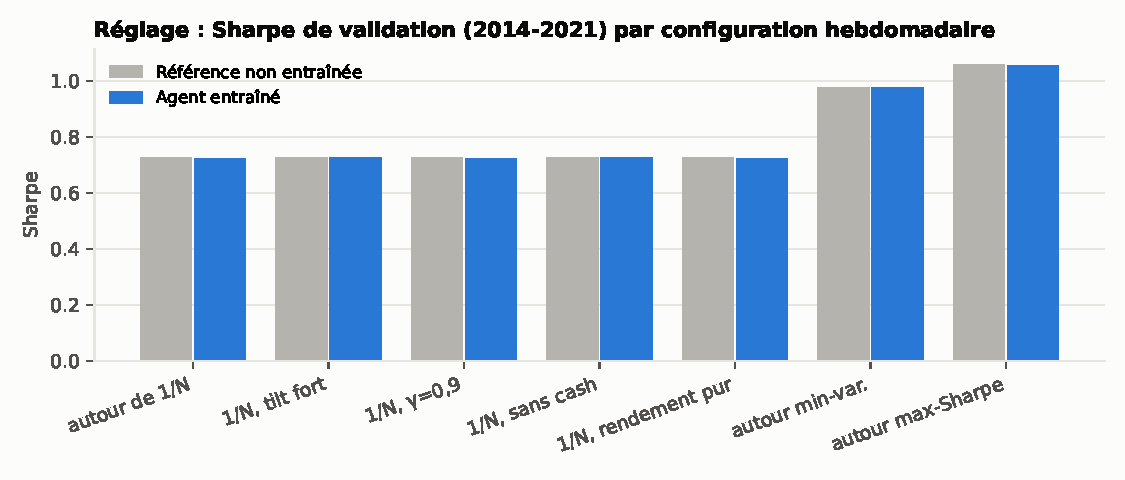
\includegraphics[width=\linewidth]{fig_reglage}
  \caption{Sharpe de validation (2014--2021) de l'agent entraîné et de sa référence non entraînée.}
  \label{fig:reglage}
\end{figure}

\subsection{Validation glissante 2014--2021}

\begin{table}[H]
\centering\small
\caption{Validation glissante (4 blocs mis bout à bout, 414 semaines).}
\begin{tabular}{@{}lrrrc@{}}
\toprule
Stratégie & Rdt/an & Sharpe & Pire perte & Sharpe par bloc (14-15 · 16-17 · 18-19 · 20-21)\\
\midrule
\textbf{Agent PPO (retenu)} & 19,75\,\% & \textbf{1,05} & \(-29{,}4\,\%\) & 0,81 · 1,34 · 1,30 · 0,97\\
Référence non entraînée & 19,98\,\% & 1,06 & \(-29{,}7\,\%\) & 0,82 · 1,34 · 1,31 · 0,97\\
Max-Sharpe & 20,75\,\% & 1,09 & \(-28{,}2\,\%\) & 0,78 · 1,35 · 1,36 · 1,05\\
Variance minimale & 15,33\,\% & 1,00 & \(-27{,}0\,\%\) & 1,21 · 1,12 · 1,45 · 0,58\\
Momentum 12-1 & 15,69\,\% & 0,83 & \(-32{,}3\,\%\) & 0,55 · 1,32 · 1,02 · 0,74\\
Faible volatilité & 12,53\,\% & 0,81 & \(-29{,}9\,\%\) & 1,16 · 0,79 · 0,98 · 0,52\\
Parité de risque & 13,78\,\% & 0,78 & \(-33{,}8\,\%\) & 0,76 · 1,26 · 0,80 · 0,62\\
1/N & 13,13\,\% & 0,72 & \(-35{,}2\,\%\) & 0,70 · 1,18 · 0,63 · 0,64\\
ETF Euro Stoxx 50 & 8,48\,\% & 0,52 & \(-33{,}8\,\%\) & 0,47 · 0,79 · 0,48 · 0,47\\
\bottomrule
\end{tabular}
\end{table}

\begin{figure}[H]
  \centering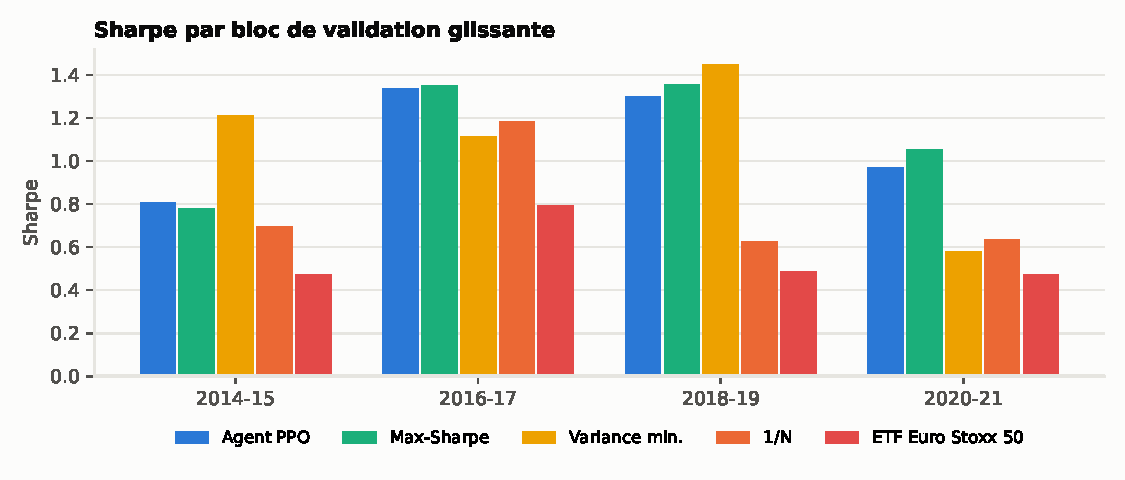
\includegraphics[width=\linewidth]{fig_validation_blocs}
  \caption{Sharpe par bloc de validation : l'agent est régulier, sans être le meilleur sur chaque bloc.}
\end{figure}

\subsection{Test final 2022--2026}

\begin{table}[H]
\centering\small
\caption{Test unique (254 semaines, frais inclus). IC95 : intervalle de confiance du Sharpe ; p : test de
différence de Sharpe avec 1/N.}
\begin{tabular}{@{}lrrrrrc@{}}
\toprule
Stratégie & Rdt/an & Volatilité & Sharpe & Pire perte & Rdt cumulé & IC95 / p\\
\midrule
\textbf{Agent PPO (ensemble)} & \textbf{16,45\,\%} & 15,66\,\% & \textbf{1,05} & \(-18{,}2\,\%\) & 110,4\,\% & [0,20 ; 1,99] / 0,88\\
Référence non entraînée & 16,58\,\% & 15,81\,\% & 1,05 & \(-18{,}3\,\%\) & 111,5\,\% & [0,20 ; 1,99] / 0,88\\
1/N & 16,29\,\% & 16,34\,\% & 1,01 & \(-17{,}0\,\%\) & 109,0\,\% & [0,14 ; 1,98] / --\\
Max-Sharpe & 15,95\,\% & 16,37\,\% & 0,99 & \(-20{,}8\,\%\) & 106,0\,\% & [0,08 ; 1,95] / 0,95\\
Variance minimale & 16,83\,\% & 11,85\,\% & 1,37 & \(-9{,}0\,\%\) & 113,8\,\% & [0,57 ; 2,24] / 0,33\\
Faible volatilité & 18,45\,\% & 13,16\,\% & 1,35 & \(-10{,}2\,\%\) & 128,7\,\% & [0,54 ; 2,20] / 0,28\\
Parité de risque & 16,44\,\% & 14,48\,\% & 1,13 & \(-14{,}6\,\%\) & 110,4\,\% & [0,26 ; 2,13] / 0,12\\
Momentum 12-1 & 22,14\,\% & 20,01\,\% & 1,10 & \(-23{,}2\,\%\) & 165,7\,\% & [0,23 ; 2,10] / 0,71\\
ETF Euro Stoxx 50 & 9,97\,\% & 16,77\,\% & 0,65 & \(-21{,}0\,\%\) & 59,1\,\% & [\(-0{,}22\) ; 1,56] / 0,00\\
Indice (prix) & 6,82\,\% & 16,63\,\% & 0,48 & \(-22{,}9\,\%\) & 38,0\,\% & [\(-0{,}38\) ; 1,40] / 0,00\\
\bottomrule
\end{tabular}
\end{table}

\begin{figure}[H]
  \centering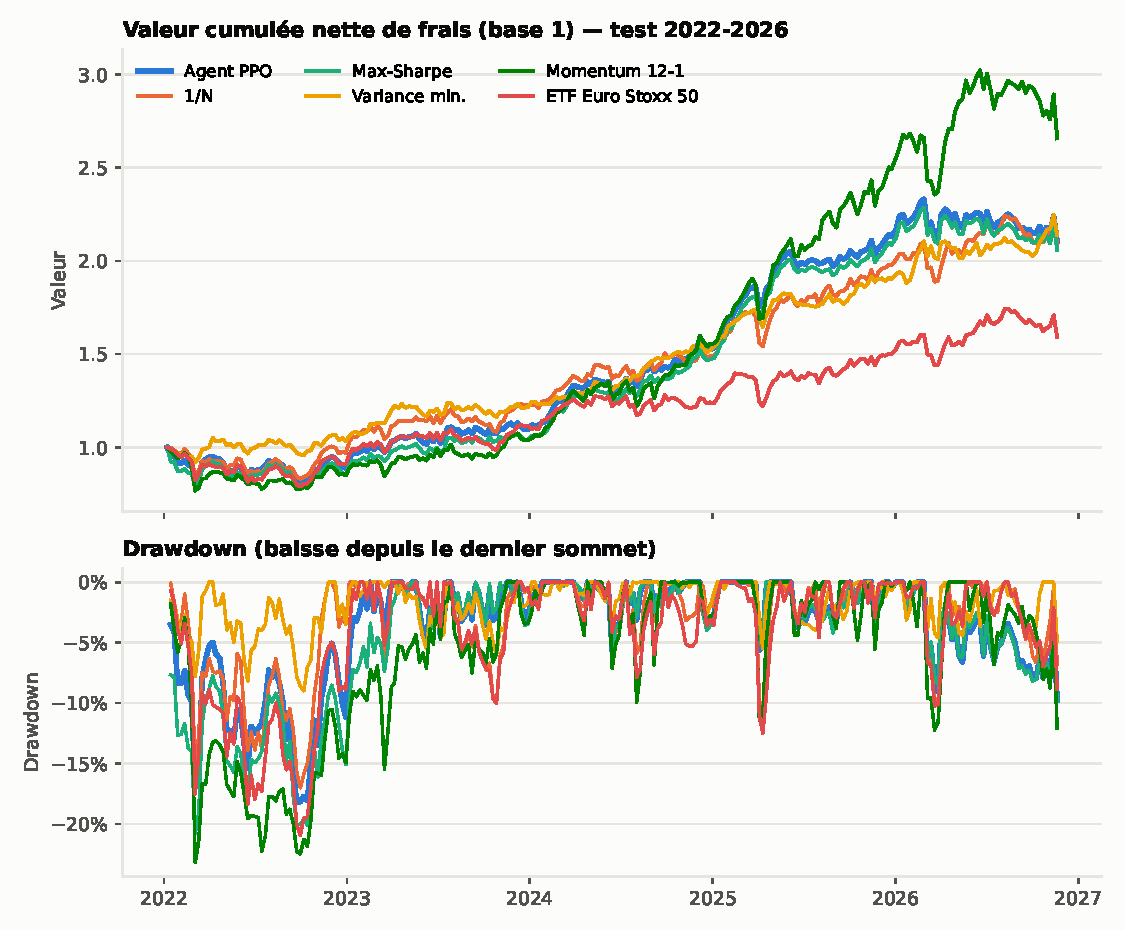
\includegraphics[width=\linewidth]{fig_test_valeur_drawdown}
  \caption{Valeur cumulée et drawdown au test. 1\,€ investi dans l'agent en janvier 2022 vaut 2,10\,€
  fin 2026, contre 1,59\,€ dans l'ETF.}
  \label{fig:valeur}
\end{figure}

\begin{figure}[H]
  \centering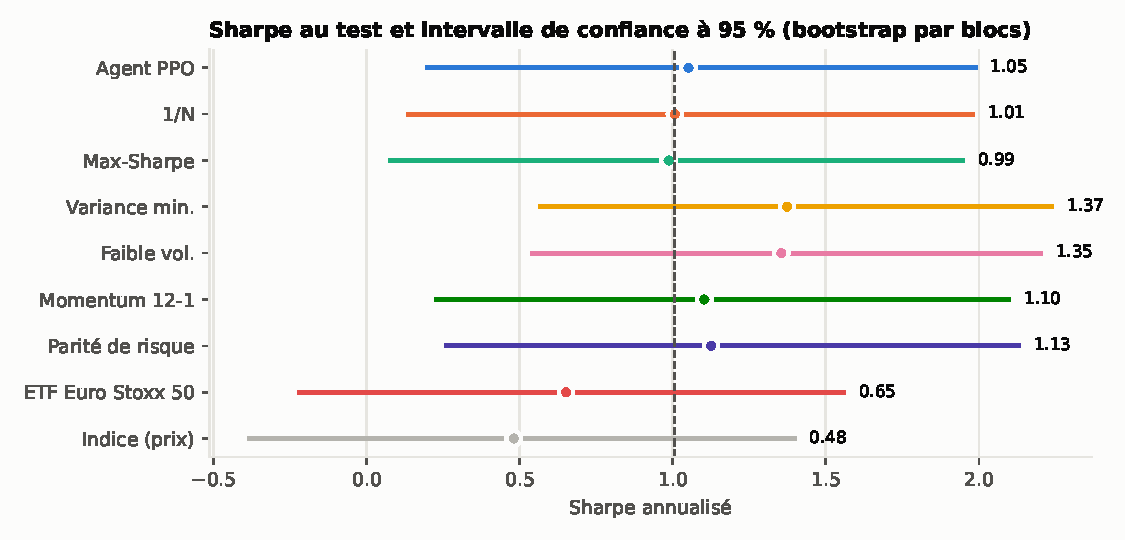
\includegraphics[width=0.92\linewidth]{fig_test_ic_sharpe}
  \caption{Sharpe au test et intervalles de confiance à 95\,\% ; la ligne pointillée indique le Sharpe de 1/N.}
  \label{fig:ic}
\end{figure}

\begin{figure}[H]
  \centering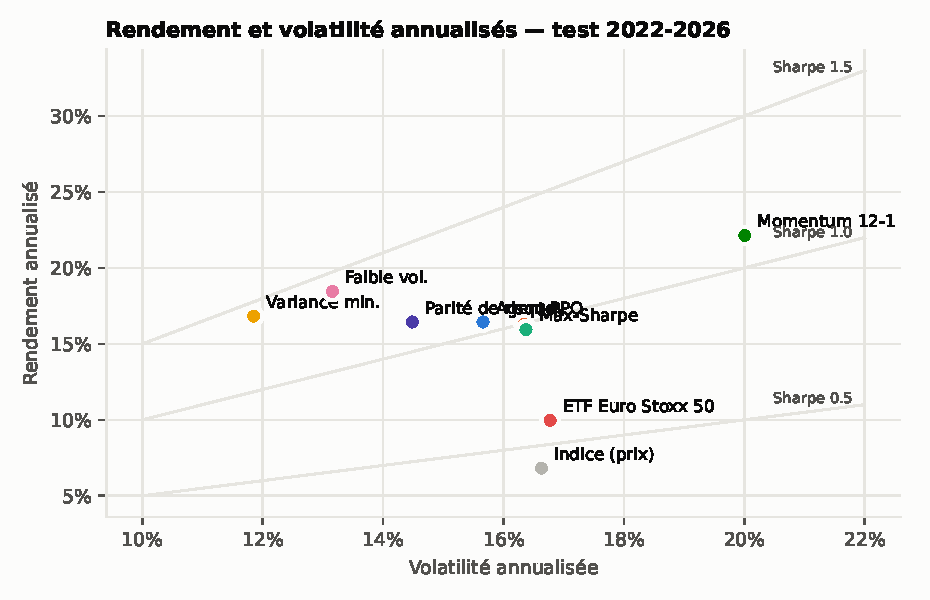
\includegraphics[width=0.8\linewidth]{fig_test_rendement_risque}
  \caption{Positionnement rendement/risque au test ; les droites grises sont des iso-Sharpe.}
\end{figure}

\subsection{Comportement de l'agent}
La figure~\ref{fig:poids} montre les poids de l'agent : il est concentré, comme sa référence max-Sharpe
(Rheinmetall, Argenx, Ahold Delhaize, UniCredit\dots), et garde en moyenne moins de 1\,\% de cash au test.
Son turnover hebdomadaire moyen (7,1\,\%) est proche de celui du max-Sharpe (7,3\,\%) et supérieur à celui de 1/N
(2,4\,\%), à cause des réestimations mensuelles de la référence (figure~\ref{fig:turnover}).

\begin{figure}[H]
  \centering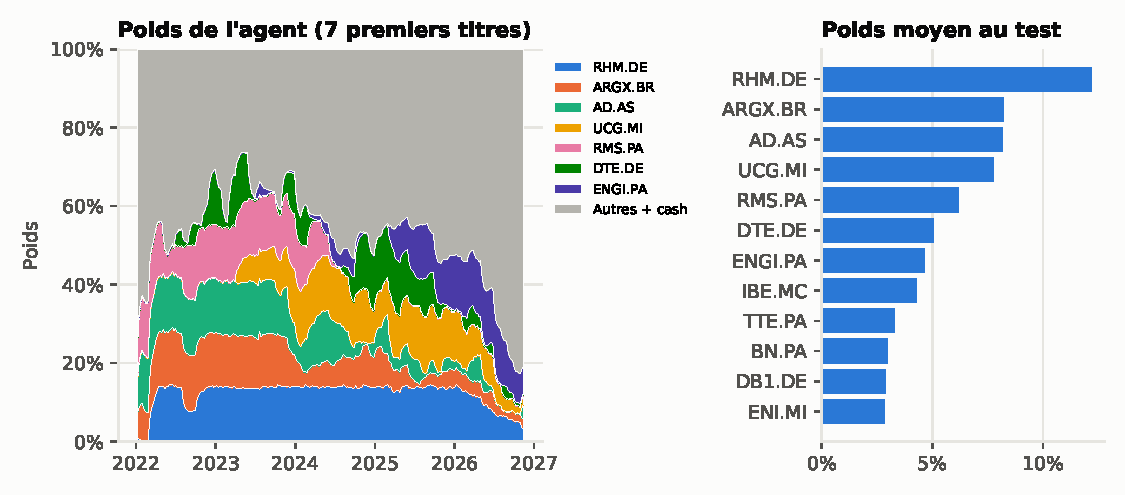
\includegraphics[width=\linewidth]{fig_poids_agent}
  \caption{Composition du portefeuille de l'agent au test et poids moyens des principaux titres.}
  \label{fig:poids}
\end{figure}

\begin{figure}[H]
  \centering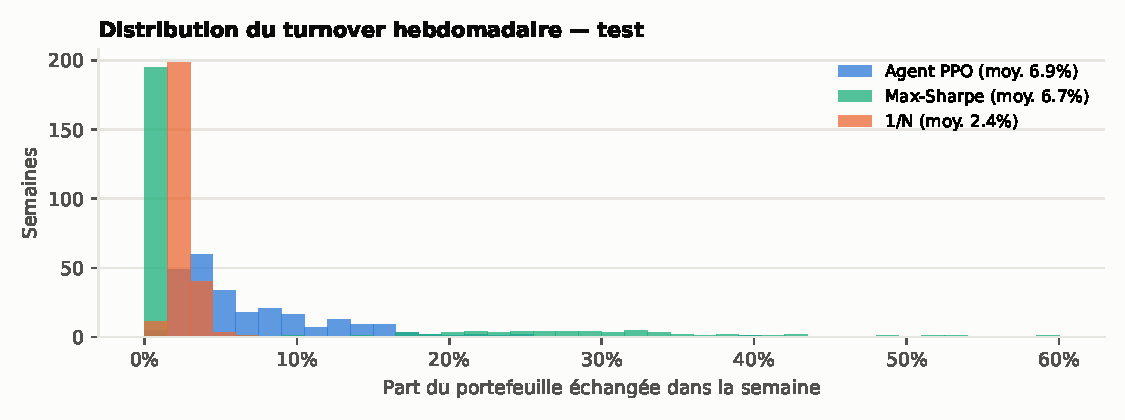
\includegraphics[width=\linewidth]{fig_turnover}
  \caption{Distribution du turnover hebdomadaire au test.}
  \label{fig:turnover}
\end{figure}

\begin{figure}[H]
  \centering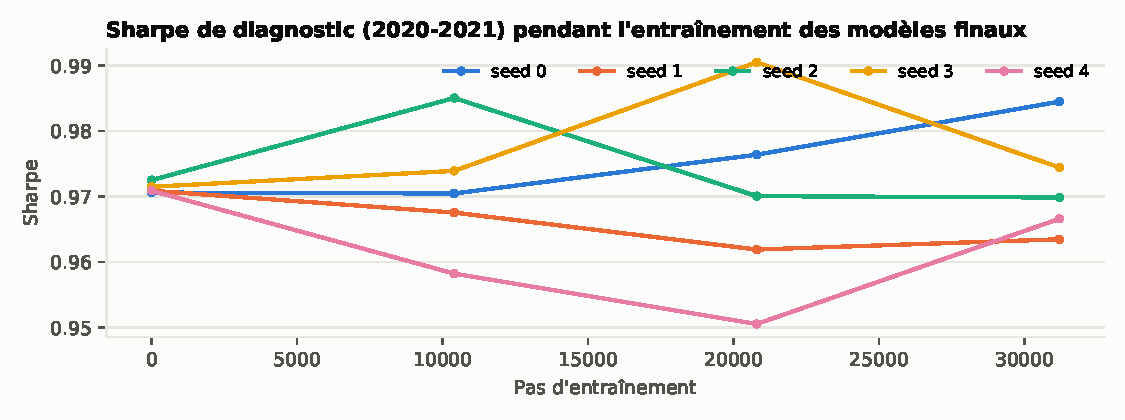
\includegraphics[width=\linewidth]{fig_entrainement}
  \caption{Sharpe de diagnostic (2020--2021) au cours de l'entraînement des 5 modèles finaux : il varie peu,
  signe que la politique reste proche de sa référence.}
\end{figure}

% =====================================================================
\section{Discussion}\label{sec:discussion}

\subsection{Ce que les résultats établissent}
\begin{itemize}
  \item L'agent \textbf{bat nettement le marché} : Sharpe 1,05 contre 0,65 pour l'ETF, et +16,5\,\%/an contre
        +10,0\,\%/an, avec une pire perte plus faible. Ce résultat est \textbf{stable} entre la validation
        (1,05) et le test (1,05).
  \item \textbf{L'apport propre de l'apprentissage est faible} : l'agent entraîné fait presque exactement comme
        sa référence non entraînée, en validation comme au test. La performance vient surtout de deux choix de
        conception : l'univers de 50 titres et le portefeuille de référence max-Sharpe.
  \item \textbf{Aucune stratégie diversifiée n'est significativement meilleure que 1/N} au test
        (p-values \(\ge0{,}12\)) : les intervalles de confiance du Sharpe sur 5 ans se recouvrent largement.
\end{itemize}

\subsection{En quoi le modèle fait-il mieux que l'ETF ?}
L'ETF Euro Stoxx 50 réplique l'indice : il détient les 50 titres en proportion de leur capitalisation boursière,
sans jamais chercher à faire mieux (gestion \emph{passive}). L'écart de rendement avec le modèle (+6,5 points par
an au test) s'explique en trois étapes, illustrées par la figure~\ref{fig:ecart} :

\begin{enumerate}
  \item \textbf{La façon de répartir l'argent entre les 50 titres (\(+6{,}3\) points).} Le simple portefeuille 1/N,
        qui met le même poids sur les 50 titres, fait déjà 16,3\,\%/an contre 10,0\,\% pour l'ETF. Un indice pondéré par
        la capitalisation concentre l'argent sur les plus grandes sociétés ; répartir plus équitablement a donné plus de
        poids à des titres plus petits qui ont fortement progressé sur 2022--2026 (banques, défense\dots).
  \item \textbf{Un effet de composition à ne pas surestimer.} L'univers est la composition \emph{actuelle} de l'indice.
        Or une société entre dans l'indice souvent \emph{parce que} son cours a fortement monté : Rheinmetall a pris
        +832\,\% entre janvier 2022 et novembre 2026, et pèse en moyenne 12\,\% du portefeuille de l'agent. Une partie de
        l'avance sur l'ETF vient donc de ce \emph{biais de survie} (voir les limites), commun à toutes les stratégies
        construites sur les 50 titres actuels.
  \item \textbf{Le choix des poids par le modèle (\(+0{,}2\) point, Sharpe \(1{,}05\) contre \(1{,}01\)).} Par rapport à
        1/N, le portefeuille de référence (max-Sharpe) puis les ajustements de l'agent améliorent un peu le
        rapport rendement/risque, sans que cet écart soit statistiquement significatif.
\end{enumerate}

\begin{figure}[H]
  \centering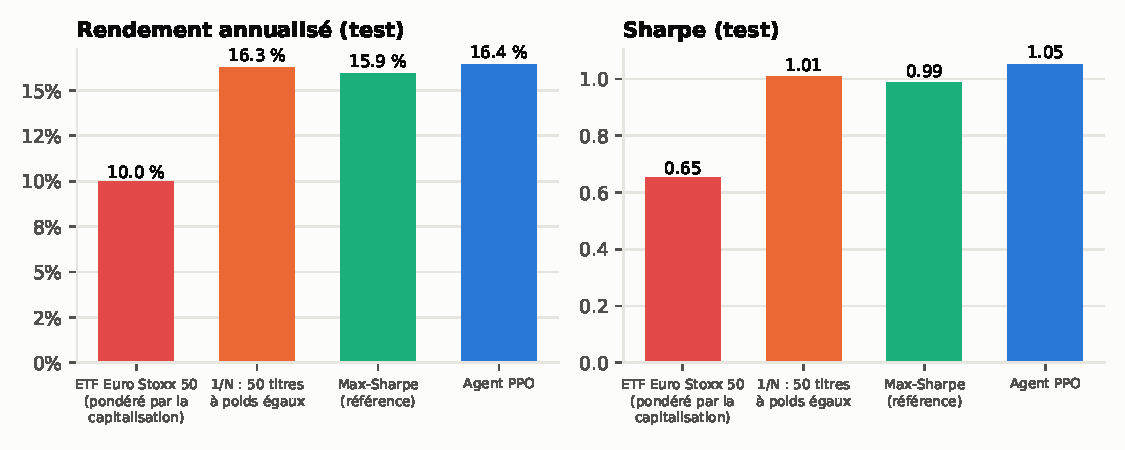
\includegraphics[width=\linewidth]{fig_ecart_etf}
  \caption{D'où vient l'écart avec l'ETF : l'essentiel vient de la répartition entre les 50 titres actuels,
  le modèle n'ajoutant qu'un gain modeste au-delà de 1/N.}
  \label{fig:ecart}
\end{figure}

\noindent Le modèle fait donc mieux que l'ETF en rendement (\(+6{,}5\) points par an), en Sharpe (\(1{,}05\) contre
\(0{,}65\)) et en perte maximale (\(-18\,\%\) contre \(-21\,\%\)). Sur cinq ans seulement, l'écart de Sharpe n'est
toutefois pas statistiquement significatif (test apparié : \(p=0{,}17\)) ; il est en revanche observé sur toutes les
périodes de validation (figure~\ref{fig:regularite}). Il faut présenter honnêtement cet avantage comme celui d'une
\emph{gestion active diversifiée sur les 50 titres}, dont l'apprentissage n'explique qu'une petite partie.

\subsection{Pourquoi retenir l'agent plutôt que le max-Sharpe ou la variance minimale ?}
Sur le test, la variance minimale (Sharpe 1,37) et la faible volatilité (1,35) ont fait mieux que l'agent (1,05).
Pourquoi ne pas les choisir ? Trois raisons.

\paragraph{1. Choisir d'après le test serait un biais.} Le test sert à \emph{mesurer} le modèle, pas à le
\emph{choisir}. La stratégie la meilleure sur une période donnée change d'une période à l'autre
(figure~\ref{fig:regularite}) : la variance minimale était la meilleure en 2018--2019 (1,45) mais l'une des pires en
2020--2021 (0,58) ; la faible volatilité, en tête au test, était parmi les dernières en 2020--2021 (0,52). De plus, au
test, ni la variance minimale ni la faible volatilité ne battent l'agent de façon statistiquement significative
(\(p=0{,}28\) et \(p=0{,}43\)). Choisir la gagnante
après coup reviendrait à parier que la même stratégie gagnera aussi la période suivante, ce que l'historique
contredit. Sur la validation (2014--2021), qui a servi à choisir, le max-Sharpe (1,09) et l'agent (1,05) étaient en
tête, devant la variance minimale (1,00).

\paragraph{2. L'agent est le plus régulier.} Sur les cinq périodes (quatre de validation et le test), l'agent a le
\textbf{meilleur Sharpe dans sa pire période} (0,81, contre 0,78 pour le max-Sharpe, 0,58 pour la variance minimale
et 0,52 pour la faible volatilité) et la plus faible dispersion des stratégies actives (écart-type de 0,22 contre
0,34 pour la variance minimale). Pour un investisseur, ne jamais connaître de « mauvaise période » est souvent plus
précieux qu'une moyenne légèrement supérieure.

\begin{figure}[H]
  \centering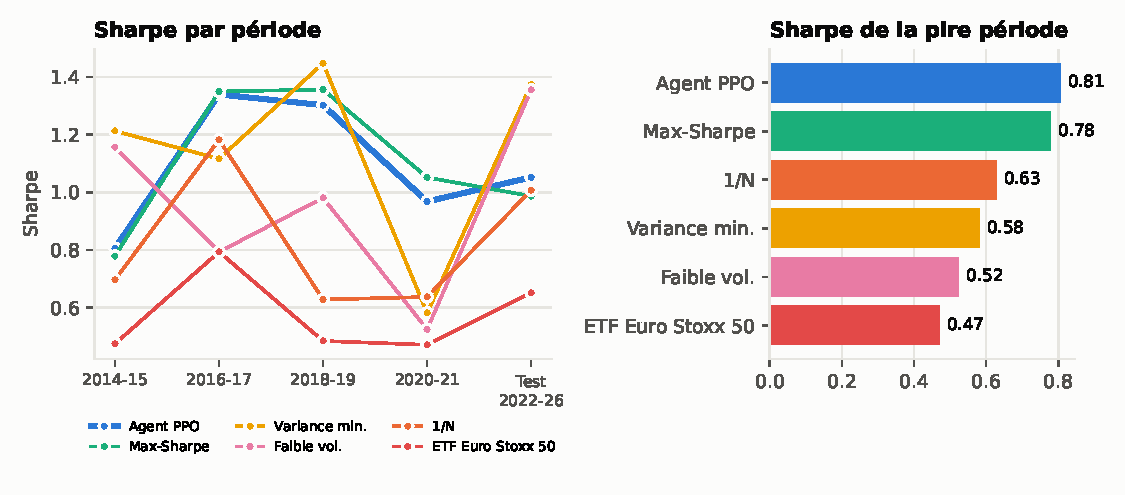
\includegraphics[width=\linewidth]{fig_regularite}
  \caption{Sharpe de chaque stratégie sur les cinq périodes (gauche) et dans sa pire période (droite).}
  \label{fig:regularite}
\end{figure}

\paragraph{3. L'agent contient le max-Sharpe et le complète.} L'agent n'est pas en concurrence avec le max-Sharpe : il
\emph{l'utilise} comme point de départ, et y ajoute des capacités qu'une règle fixe n'a pas : réagir chaque semaine aux
signaux des titres et au contexte de marché, et mettre jusqu'à 50\,\% en cash en période de stress, tout en limitant
les frais par le lissage. Sur nos données, ces capacités ont peu servi (l'agent reste proche de sa référence), mais
elles sont en place, testées, et pourraient être mieux exploitées avec davantage d'informations
(section~\ref{sec:limites}).

\paragraph{Et les gérants professionnels ?} Les fonds qui « gèrent l'Euro Stoxx 50 » sont pour la plupart des ETF
passifs qui répliquent l'indice pondéré par la capitalisation : c'est la référence que nous battons. Il existe aussi des
fonds dits \emph{smart beta} qui appliquent précisément les règles de nos stratégies de référence (poids égaux,
variance minimale, faible volatilité\dots) : dans notre comparaison, aucune de ces règles ne bat l'agent de façon
statistiquement significative, et aucune n'est aussi régulière d'une période à l'autre.

\paragraph{En résumé.} Si l'objectif était uniquement de maximiser le Sharpe passé sur 2022--2026, la variance minimale
aurait été le meilleur choix \emph{a posteriori}. L'objectif de ce projet était de construire un système d'allocation
dynamique par apprentissage par renforcement, choisi selon un protocole sans biais : l'agent retenu est le meilleur
système RL en validation, le plus régulier de toutes les stratégies, et nettement supérieur à l'ETF.

\subsection{Pourquoi cette conception : alternatives étudiées}
Le modèle retenu est l'aboutissement de plusieurs approches, évaluées avec le même protocole et sélectionnées
sur la validation, jamais sur le test (tableau~\ref{tab:versions}, figure~\ref{fig:versions}).

\begin{table}[H]
\centering\small
\caption{Approches explorées (Sharpe au test 2022--2026, donné à titre indicatif).}
\label{tab:versions}
\begin{tabularx}{\linewidth}{@{}lYc@{}}
\toprule
Approche & Constat & Sharpe test\\
\midrule
PPO, 20 titres, 30 rendements bruts par titre & sur-apprentissage : la récompense d'entraînement monte, la validation baisse & 0,58\\
PPO bridé (rangs, réseau partagé, lissage) & n'apprend plus rien, reste sur 1/N & \(\approx\)1/N\\
PPO pour l'exposition actions/cash & réduit le risque, mais une exposition fixe à 50\,\% fait aussi bien & 0,73\\
\textbf{PPO, 50 titres, autour du max-Sharpe} & \textbf{retenu : meilleur en validation, stable} & \textbf{1,05}\\
Gradient direct (backtest différentiable) & apprend en validation (+0,17), pas au test & 0,93\\
PPO répartissant entre 6 stratégies & décisions actives, sans gain sur le mélange égal & 1,18\\
\bottomrule
\end{tabularx}
\end{table}

\begin{figure}[H]
  \centering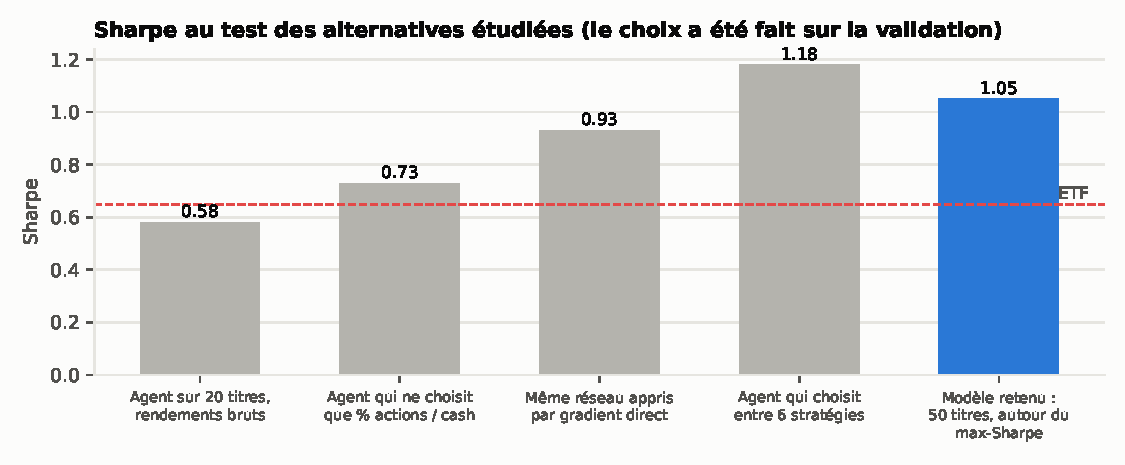
\includegraphics[width=\linewidth]{fig_versions}
  \caption{Sharpe au test des approches explorées. Le choix du modèle final s'est fait sur la validation :
  retenir a posteriori la meilleure approche au test serait un biais de sélection.}
  \label{fig:versions}
\end{figure}

\paragraph{Pourquoi l'agent apprend peu.} Une expérience de contrôle sur un marché synthétique, où un signal
prédictif a été volontairement caché, montre que PPO retrouve ce signal quand il est assez fort (Sharpe hors
échantillon de 0,34 contre \(-1{,}36\) pour l'action nulle), aussi bien qu'une méthode à gradient exact. La
limite ne vient donc pas de l'algorithme, mais du \textbf{faible signal exploitable} dans les prix passés à
horizon hebdomadaire : le bruit des rendements domine l'effet des bonnes décisions.

% =====================================================================
\section{Architecture logicielle}

\subsection{Organisation et flux de données}
Le code est organisé en modules indépendants (dossier \texttt{src/}) pilotés par deux scripts ; tous les
paramètres sont dans \texttt{config.yaml} (aucune valeur codée en dur). La figure~\ref{fig:pipeline} décrit le
flux complet.

\begin{figure}[H]
\centering
\begin{tikzpicture}[node distance=0.55cm, >=Stealth, every node/.style={font=\footnotesize},
  m/.style={draw=bleu, fill=fond, rounded corners, align=center, minimum width=2.6cm, minimum height=1.0cm, thick},
  d/.style={draw=gris, fill=white, align=center, minimum width=2.6cm, minimum height=0.8cm, dashed}]
  \node[d] (wiki) {Wikipédia\\ Yahoo Finance};
  \node[m, right=of wiki] (data) {\texttt{data.py}\\ tickers, nettoyage};
  \node[m, right=of data] (uni) {\texttt{universe.py}\\ signaux, masque};
  \node[m, right=of uni] (env) {\texttt{env.py}\\ MDP, comptabilité};
  \node[m, below=1.1cm of env] (train) {\texttt{train.py} + \texttt{policies.py}\\ PPO, réseau partagé};
  \node[m, left=of train] (base) {\texttt{baselines.py}\\ stratégies (cvxpy)};
  \node[m, left=of base] (eval) {\texttt{metrics.py}, \texttt{evaluate.py}\\ \texttt{plots.py}};
  \node[d, left=of eval] (res) {\texttt{results/}\\ tables, figures, modèles};
  \draw[->, thick] (wiki) -- (data); \draw[->, thick] (data) -- (uni); \draw[->, thick] (uni) -- (env);
  \draw[->, thick] (env) -- (train); \draw[->, thick] (train) -- (base);
  \draw[->, thick] (base) -- (eval); \draw[->, thick] (eval) -- (res);
  \node[above=0.15cm of data, gris] {\texttt{scripts/01\_download\_data.py}};
  \node[below=0.15cm of base, gris] {\texttt{scripts/02\_train\_evaluate.py}};
\end{tikzpicture}
\caption{Flux de données et modules du projet.}
\label{fig:pipeline}
\end{figure}

\begin{table}[H]
\centering\small
\caption{Rôle des modules.}
\begin{tabularx}{\linewidth}{@{}lY@{}}
\toprule
Fichier & Rôle\\
\midrule
\texttt{config.yaml} & tous les paramètres : données, signaux, environnement, PPO, protocole, métriques\\
\texttt{src/data.py} & scraping Wikipédia, conversion en tickers Yahoo, téléchargement, nettoyage, rapport\\
\texttt{src/universe.py} & univers dynamique, signaux par titre, contexte de marché, normalisation train-only\\
\texttt{src/features.py} & calendrier hebdomadaire, découpage temporel, structure \texttt{MarketData}\\
\texttt{src/env.py} & environnement Gymnasium : actions\(\to\)poids, coûts, dérive, récompense, masque\\
\texttt{src/policies.py} & politique PPO à réseau partagé entre titres (équivariante, masquée)\\
\texttt{src/train.py} & fabriques d'agents (PPO ; A2C, SAC, TD3 prévus avec la même interface), entraînement\\
\texttt{src/baselines.py} & stratégies de référence (variance minimale, max-Sharpe, parité de risque\dots)\\
\texttt{src/metrics.py} & métriques de performance, bootstrap du Sharpe, test de différence\\
\texttt{src/evaluate.py}, \texttt{plots.py} & tableaux CSV/Markdown, verrou du test final, figures\\
\texttt{scripts/01\_download\_data.py} & étape données (cache dans \texttt{data/raw})\\
\texttt{scripts/02\_train\_evaluate.py} & réglage (\texttt{--tune}) et test final (\texttt{--final-test})\\
\texttt{tests/} & 25 tests automatiques (pytest)\\
\bottomrule
\end{tabularx}
\end{table}

\subsection{Le code pas à pas}
Cette section suit le chemin d'une exécution complète, avec des extraits du code réel (commentaires traduits et
simplifiés).

\paragraph{Étape 1 : les données (\texttt{scripts/01\_download\_data.py}).} Le script lit la composition de l'indice sur
Wikipédia, convertit chaque société en ticker Yahoo, télécharge les prix, les nettoie et les met en cache dans
\texttt{data/}. Il écrit aussi un rapport (\texttt{data/processed/report.md}).

\paragraph{Étape 2 : les informations de l'agent (\texttt{src/universe.py}).} La fonction \texttt{build\_market\_data}
calcule, pour chaque vendredi et chaque titre, les 14 informations de la section~\ref{sec:etat}, le masque de disponibilité
et les rendements de la semaine suivante. Tout est rangé dans un objet \texttt{MarketData} (tableaux NumPy de
dimensions semaines \(\times\) titres \(\times\) informations), partagé par l'agent et les stratégies de référence.
Les rangs ne sont calculés que parmi les titres disponibles :

\begin{lstlisting}
def masked_rank(df):
    """Rang dans [-1, 1] parmi les titres disponibles a chaque date (NaN = titre indisponible)."""
    n = df.notna().sum(axis=1)
    r = df.rank(axis=1)
    return (r - 1.0).div((n - 1).where(n > 1), axis=0) * 2.0 - 1.0
\end{lstlisting}

\paragraph{Étape 3 : l'environnement (\texttt{src/env.py}).} La classe \texttt{PortfolioEnv} suit l'interface
Gymnasium : \texttt{reset()} démarre un épisode, \texttt{step(action)} joue une semaine. La conversion de l'action en
poids (section~\ref{sec:action}) tient en quelques lignes :

\begin{lstlisting}
def action_to_weights(self, action):
    a = np.clip(action, -1.0, 1.0)                     # notes dans [-1, 1]
    m = self.mask()                                     # titres disponibles cette semaine
    cash = self.cash_max * max(a[-1], 0.0)              # part de cash (0 a 50 %)
    logits = self.residual_scale * a[:-1][m]            # notes des titres disponibles
    logits += np.log(self._base[self.current_k][m] + self.base_floor)   # decalage par la reference
    risky = np.zeros(self.md.n_assets)
    risky[m] = softmax(logits)                          # repartition entre titres (somme 1)
    return np.append((1.0 - cash) * risky, cash)
\end{lstlisting}

\noindent puis l'exécution d'une semaine applique le lissage, la comptabilité commune et calcule la récompense :

\begin{lstlisting}
def step_target(self, target):
    k = self.current_k
    w_new = (1 - self.alpha) * self._weights + self.alpha * target      # lissage
    res = rebalance_step(self._weights, w_new, self.md.weekly_returns[k],
                         self.cost_rate, self.turnover_includes_cash)   # frais, derive
    reward = (res.gross_return - self.reward_cost_rate * res.turnover
              - 0.5 * self.risk_aversion * res.net_return ** 2) * self.reward_scale
    self._weights = res.drifted_weights                                 # poids de la semaine suivante
    ...
\end{lstlisting}

\paragraph{Étape 4 : le réseau (\texttt{src/policies.py}).} La classe \texttt{SharedAssetNet} implémente les
équations de la section~\ref{sec:reseau} ; la note de chaque titre est calculée par le même réseau \texttt{embed} :

\begin{lstlisting}
def forward_actor(self, obs):
    feats = obs[:, :N*F].reshape(B, N, F)                # 14 informations par titre
    w = obs[:, N*F:]                                     # poids courants (+ cash)
    e = self.embed(torch.cat([feats, w[:, :N, None]], -1))   # meme reseau pour chaque titre
    m = feats[:, :, -1:]                                 # drapeau de disponibilite
    context = (e * m).sum(1) / m.sum(1).clamp(min=1)     # moyenne sur les titres disponibles
    return torch.cat([self.score(e).squeeze(-1),         # note de chaque titre
                      self.cash_head(torch.cat([context, w[:, N:]], -1))], -1)   # note du cash
\end{lstlisting}

\paragraph{Étape 5 : l'entraînement (\texttt{src/train.py}).} La fonction \texttt{train\_agent} crée l'environnement
d'entraînement, construit l'agent PPO de stable-baselines3 avec ce réseau et les hyperparamètres de
\texttt{config.yaml}, puis lance \texttt{model.learn(40\_000)} et sauvegarde le modèle
(\texttt{final\_model.zip}).

\paragraph{Étape 6 : le réglage et le test (\texttt{scripts/02\_train\_evaluate.py}).} Avec \texttt{--tune}, le
script entraîne les 8 configurations sur les 4 blocs de validation et écrit le classement
(\texttt{results/tables/tuning\_summary.md}). Avec \texttt{--final-test}, il entraîne les 5 agents finaux, les fait
jouer ensemble sur 2022--2026 en moyennant leurs poids à chaque semaine, simule les stratégies de référence dans
les mêmes conditions, puis écrit les tableaux, les figures et le verrou :

\begin{lstlisting}
def ensemble_rollout(env, acts):
    obs, _ = env.reset(seed=0)
    while not done:
        target = np.mean([env.action_to_weights(act(obs)) for act in acts], axis=0)  # moyenne des 5 agents
        obs, _, term, trunc, info = env.step_target(target)
        ...
\end{lstlisting}

\subsection{Bibliothèques}

\begin{table}[H]
\centering\small
\caption{Bibliothèques utilisées (versions figées dans \texttt{requirements.txt}, Python 3.13).}
\begin{tabularx}{\linewidth}{@{}llY@{}}
\toprule
Bibliothèque & Version & Usage\\
\midrule
stable-baselines3 \cite{sb3} & 2.9.2 & implémentation de PPO, vectorisation, moniteurs\\
PyTorch & 2.15.0 (CPU) & réseaux de neurones (politique, valeur)\\
Gymnasium \cite{gymnasium} & 1.4.0 & interface standard de l'environnement\\
yfinance & 1.8.0 & données de marché Yahoo Finance\\
pandas / NumPy & 3.1.1 / 2.5.5 & manipulation des séries temporelles, calcul vectoriel\\
SciPy / scikit-learn & 1.18.1 / 1.9.1 & statistiques ; covariance Ledoit--Wolf\\
CVXPY \cite{cvxpy} + Clarabel & 1.9.3 / 0.11.1 & optimisation convexe des stratégies de référence\\
Matplotlib & 3.11.2 & figures\\
lxml, requests, BeautifulSoup & -- & lecture de la page Wikipédia\\
PyYAML & 6.0.4 & lecture de la configuration\\
pytest & 9.2.0 & tests automatiques\\
\bottomrule
\end{tabularx}
\end{table}

\subsection{Tests et reproductibilité}
Les 25 tests vérifient notamment :
\begin{itemize}
  \item la \textbf{comptabilité} : turnover, frais (jambe cash gratuite), dérive des poids, rendement du cash ;
  \item l'\textbf{absence de look-ahead} : modifier les prix futurs ne change aucune feature passée ;
  \item l'\textbf{univers dynamique} : un titre n'est investissable qu'après 252 jours de cotation, il a un poids
        nul avant, et le bruit d'augmentation ne touche jamais le drapeau de disponibilité ;
  \item le \textbf{réseau} : changer les features d'un titre indisponible ne modifie aucune autre décision ;
  \item les \textbf{optimiseurs} (solutions analytiques connues), le \textbf{bootstrap} et le \textbf{verrou} du test.
\end{itemize}
Les données sont mises en cache : avec les modèles fournis, la commande
\texttt{python scripts/02\_train\_evaluate.py --final-test --force} reproduit exactement les résultats de ce
rapport (écart nul vérifié), en environ deux minutes.

% =====================================================================
\section{Limites et perspectives}\label{sec:limites}

\paragraph{Limites.}
\begin{itemize}
  \item \textbf{Biais de survie} : l'univers est la composition \emph{actuelle} de l'indice ; les sociétés
        sorties depuis 2009 sont absentes, ce qui flatte les performances absolues de toutes les stratégies.
  \item \textbf{Incertitude statistique} : environ dix ans d'entraînement et cinq ans de test ; les écarts entre
        stratégies diversifiées ne sont pas significatifs. Le test a été observé lors des approches successives :
        ses chiffres sont indicatifs.
  \item \textbf{Apport limité de l'apprentissage} : l'agent reste proche de sa référence.
  \item \textbf{Frais simplifiés} : coût proportionnel de 0,1\,\%, exécution au cours de clôture, sans impact de
        marché ni taxe sur les transactions ; cash rémunéré à 0\,\%.
  \item \textbf{Données Yahoo Finance} : prix ajustés rétroactivement ; benchmark avec dividendes approché par un ETF.
\end{itemize}

\paragraph{Perspectives.} Les expériences suggèrent que le levier principal est l'\emph{information} fournie à
l'agent plutôt que l'algorithme : données fondamentales (valorisation, révisions de bénéfices), variables
macroéconomiques (taux, spreads de crédit), cash rémunéré au taux réel, compositions historiques de l'indice
(pour supprimer le biais de survie), ou entraînement sur plusieurs marchés et plusieurs décennies pour
multiplier les régimes observés.

% =====================================================================
\section{Conclusion}
Ce projet a construit, de bout en bout et de manière reproductible, un système d'allocation dynamique par
apprentissage par renforcement sur les 50 actions de l'Euro Stoxx 50 : données nettoyées et univers
dynamique, environnement Gymnasium avec comptabilité réaliste, agent PPO à réseau partagé, protocole de
validation glissante et test unique verrouillé, évaluation statistique. Le modèle final obtient un Sharpe de
1,05 et un rendement de 16,5\,\%/an sur 2022--2026, nettement au-dessus de l'ETF Euro Stoxx 50. L'analyse
critique montre que ce résultat repose surtout sur la conception du problème et que, sur ces données de prix,
l'agent apprend peu au-delà de son portefeuille de référence. Cette conclusion, établie avec un protocole
rigoureux, est elle-même un résultat : elle indique où chercher pour aller plus loin.

% =====================================================================
\begin{thebibliography}{99}\small
\bibitem{schulman2017ppo} J. Schulman, F. Wolski, P. Dhariwal, A. Radford, O. Klimov. \emph{Proximal Policy Optimization Algorithms}. arXiv:1707.06347, 2017.
\bibitem{schulman2016gae} J. Schulman, P. Moritz, S. Levine, M. Jordan, P. Abbeel. \emph{High-Dimensional Continuous Control Using Generalized Advantage Estimation}. ICLR, 2016.
\bibitem{jiang2017} Z. Jiang, D. Xu, J. Liang. \emph{A Deep Reinforcement Learning Framework for the Financial Portfolio Management Problem}. arXiv:1706.10059, 2017.
\bibitem{demiguel2009} V. DeMiguel, L. Garlappi, R. Uppal. \emph{Optimal Versus Naive Diversification: How Inefficient is the 1/N Portfolio Strategy?} Review of Financial Studies, 22(5), 2009.
\bibitem{ledoitwolf2004} O. Ledoit, M. Wolf. \emph{A Well-Conditioned Estimator for Large-Dimensional Covariance Matrices}. Journal of Multivariate Analysis, 88(2), 2004.
\bibitem{spinu2013} F. Spinu. \emph{An Algorithm for Computing Risk Parity Weights}. SSRN, 2013.
\bibitem{jegadeesh1993} N. Jegadeesh, S. Titman. \emph{Returns to Buying Winners and Selling Losers}. Journal of Finance, 48(1), 1993.
\bibitem{lo2002} A. Lo. \emph{The Statistics of Sharpe Ratios}. Financial Analysts Journal, 58(4), 2002.
\bibitem{sb3} A. Raffin et al. \emph{Stable-Baselines3: Reliable Reinforcement Learning Implementations}. JMLR, 22(268), 2021.
\bibitem{gymnasium} M. Towers et al. \emph{Gymnasium: A Standard Interface for Reinforcement Learning Environments}. arXiv:2407.17032, 2024.
\bibitem{cvxpy} S. Diamond, S. Boyd. \emph{CVXPY: A Python-Embedded Modeling Language for Convex Optimization}. JMLR, 17(83), 2016.
\end{thebibliography}

% =====================================================================
\appendix
\section{Exécution}
\begin{lstlisting}[language=bash]
py -3.13 -m venv .venv
.venv/Scripts/python -m pip install torch==2.15.0 --index-url https://download.pytorch.org/whl/cpu
.venv/Scripts/python -m pip install -r requirements.txt
.venv/Scripts/python -m pytest                                        # 25 tests
.venv/Scripts/python scripts/01_download_data.py                      # donnees (cache)
.venv/Scripts/python scripts/02_train_evaluate.py --final-test --force # rejoue le test (~2 min)
.venv/Scripts/python scripts/02_train_evaluate.py --tune              # reglage complet (~2 h 15)
.venv/Scripts/python report/make_figures.py                           # figures du rapport
\end{lstlisting}

\end{document}
